% !TEX TS-program = pdflatex
% !TEX encoding = UTF-8 Unicode

% This is a simple template for a LaTeX document using the "article" class.
% See "book", "report", "letter" for other types of document.

\documentclass[11pt]{article} % use larger type; default would be 10pt


\usepackage{ulem}
\newcommand\NoIndent[1]{%
  \par\vbox{\parbox[t]{\linewidth}{#1}}%
}


\usepackage[utf8]{inputenc} % set input encoding (not needed with XeLaTeX)

%%% Examples of Article customizations
% These packages are optional, depending whether you want the features they provide.
% See the LaTeX Companion or other references for full information.

%%% PAGE DIMENSIONS
\usepackage{geometry} % to change the page dimensions
\geometry{a4paper} % or letterpaper (US) or a5paper or....
% \geometry{margin=2in} % for example, change the margins to 2 inches all round
% \geometry{landscape} % set up the page for landscape
%   read geometry.pdf for detailed page layout information

\usepackage{graphicx} % support the \includegraphics command and options

% \usepackage[parfill]{parskip} % Activate to begin paragraphs with an empty line rather than an indent

%%% PACKAGES
\usepackage{booktabs} % for much better looking tables
\usepackage{array} % for better arrays (eg matrices) in maths
\usepackage{paralist} % very flexible & customisable lists (eg. enumerate/itemize, etc.)
\usepackage{verbatim} % adds environment for commenting out blocks of text & for better verbatim
\usepackage{subfig} % make it possible to include more than one captioned figure/table in a single float
% These packages are all incorporated in the memoir class to one degree or another...

%%% HEADERS & FOOTERS
\usepackage{fancyhdr} % This should be set AFTER setting up the page geometry
\pagestyle{fancy} % options: empty , plain , fancy
\renewcommand{\headrulewidth}{0pt} % customise the layout...
\lhead{}\chead{}\rhead{}
\lfoot{}\cfoot{\thepage}\rfoot{}

%%% SECTION TITLE APPEARANCE
\usepackage{sectsty}
\allsectionsfont{\sffamily\mdseries\upshape} % (See the fntguide.pdf for font help)
% (This matches ConTeXt defaults)

%%% ToC (table of contents) APPEARANCE
\usepackage[nottoc,notlof,notlot]{tocbibind} % Put the bibliography in the ToC
\usepackage[titles,subfigure]{tocloft} % Alter the style of the Table of Contents
\renewcommand{\cftsecfont}{\rmfamily\mdseries\upshape}
\renewcommand{\cftsecpagefont}{\rmfamily\mdseries\upshape} % No bold!

%%% END Article customizations


\usepackage{verbatim}
\usepackage{amsmath}


\title{Work Log for November}
\author{Logan Brown}
%\date{} % Activate to display a given date or no date (if empty),
         % otherwise the current date is printed 

\begin{document}
\maketitle
\tableofcontents

\newpage


\section{Goals for the Month}
As of October 31st
\begin{enumerate}
\item Use Preston's Simulated Yeast, compare to REU yeast

look for estimated $\approx$ 4*true
\item Parallelize the Code

mclapply, getOption(``mc.cores")?
\item Wei Chen's Yeast / Real Yeast Genome
\item Generate my own simulated yeast, using a reverse engineered cubfits
\end{enumerate}

%Paste output from writeGoals
\section{Progress/Notes}

\subsection{Use Preston's Simulated Yeast, compare to REU yeast}

Here are the results from Preston's simulated yeast...

Notice that the $\Delta\omega$ values are not off by that $\approx4$ factor. We got a pretty good correlation on the log$\mu$ values, but the $\phi$ is pretty lousy, and the $\omega$ values leave something to be desired.

%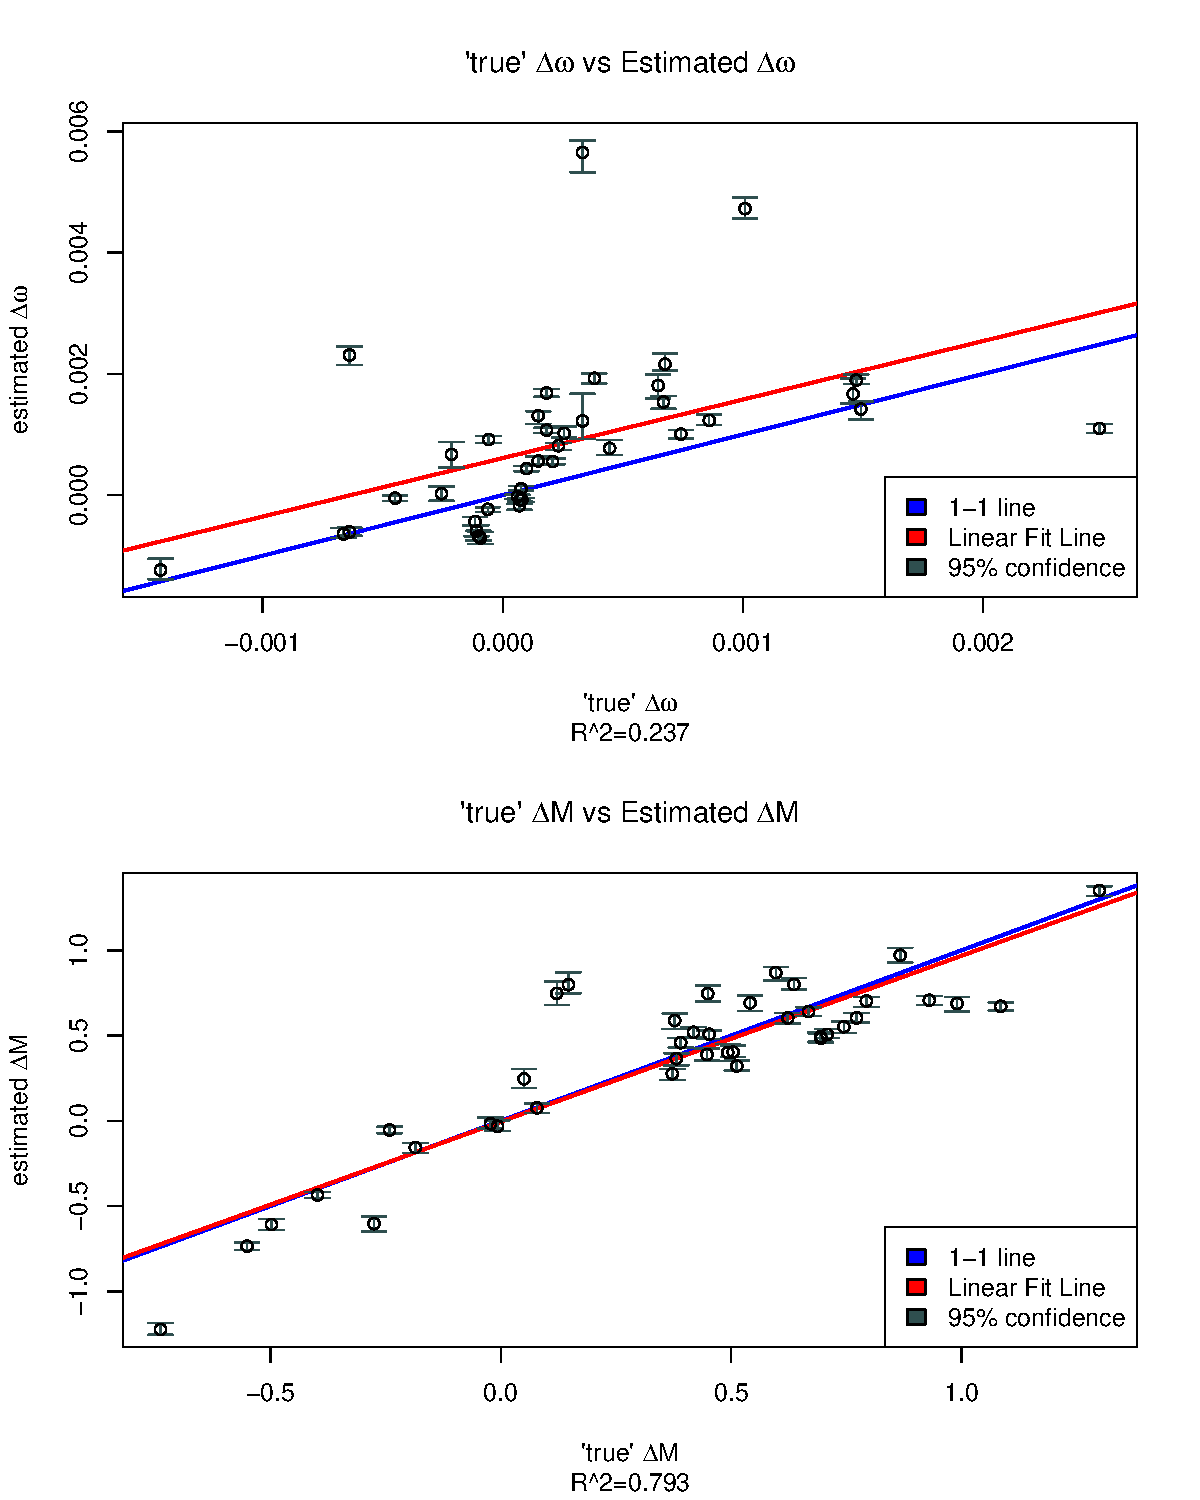
\includepdf[pages={1}]{data/1105_codonParameters_8core.pdf}
%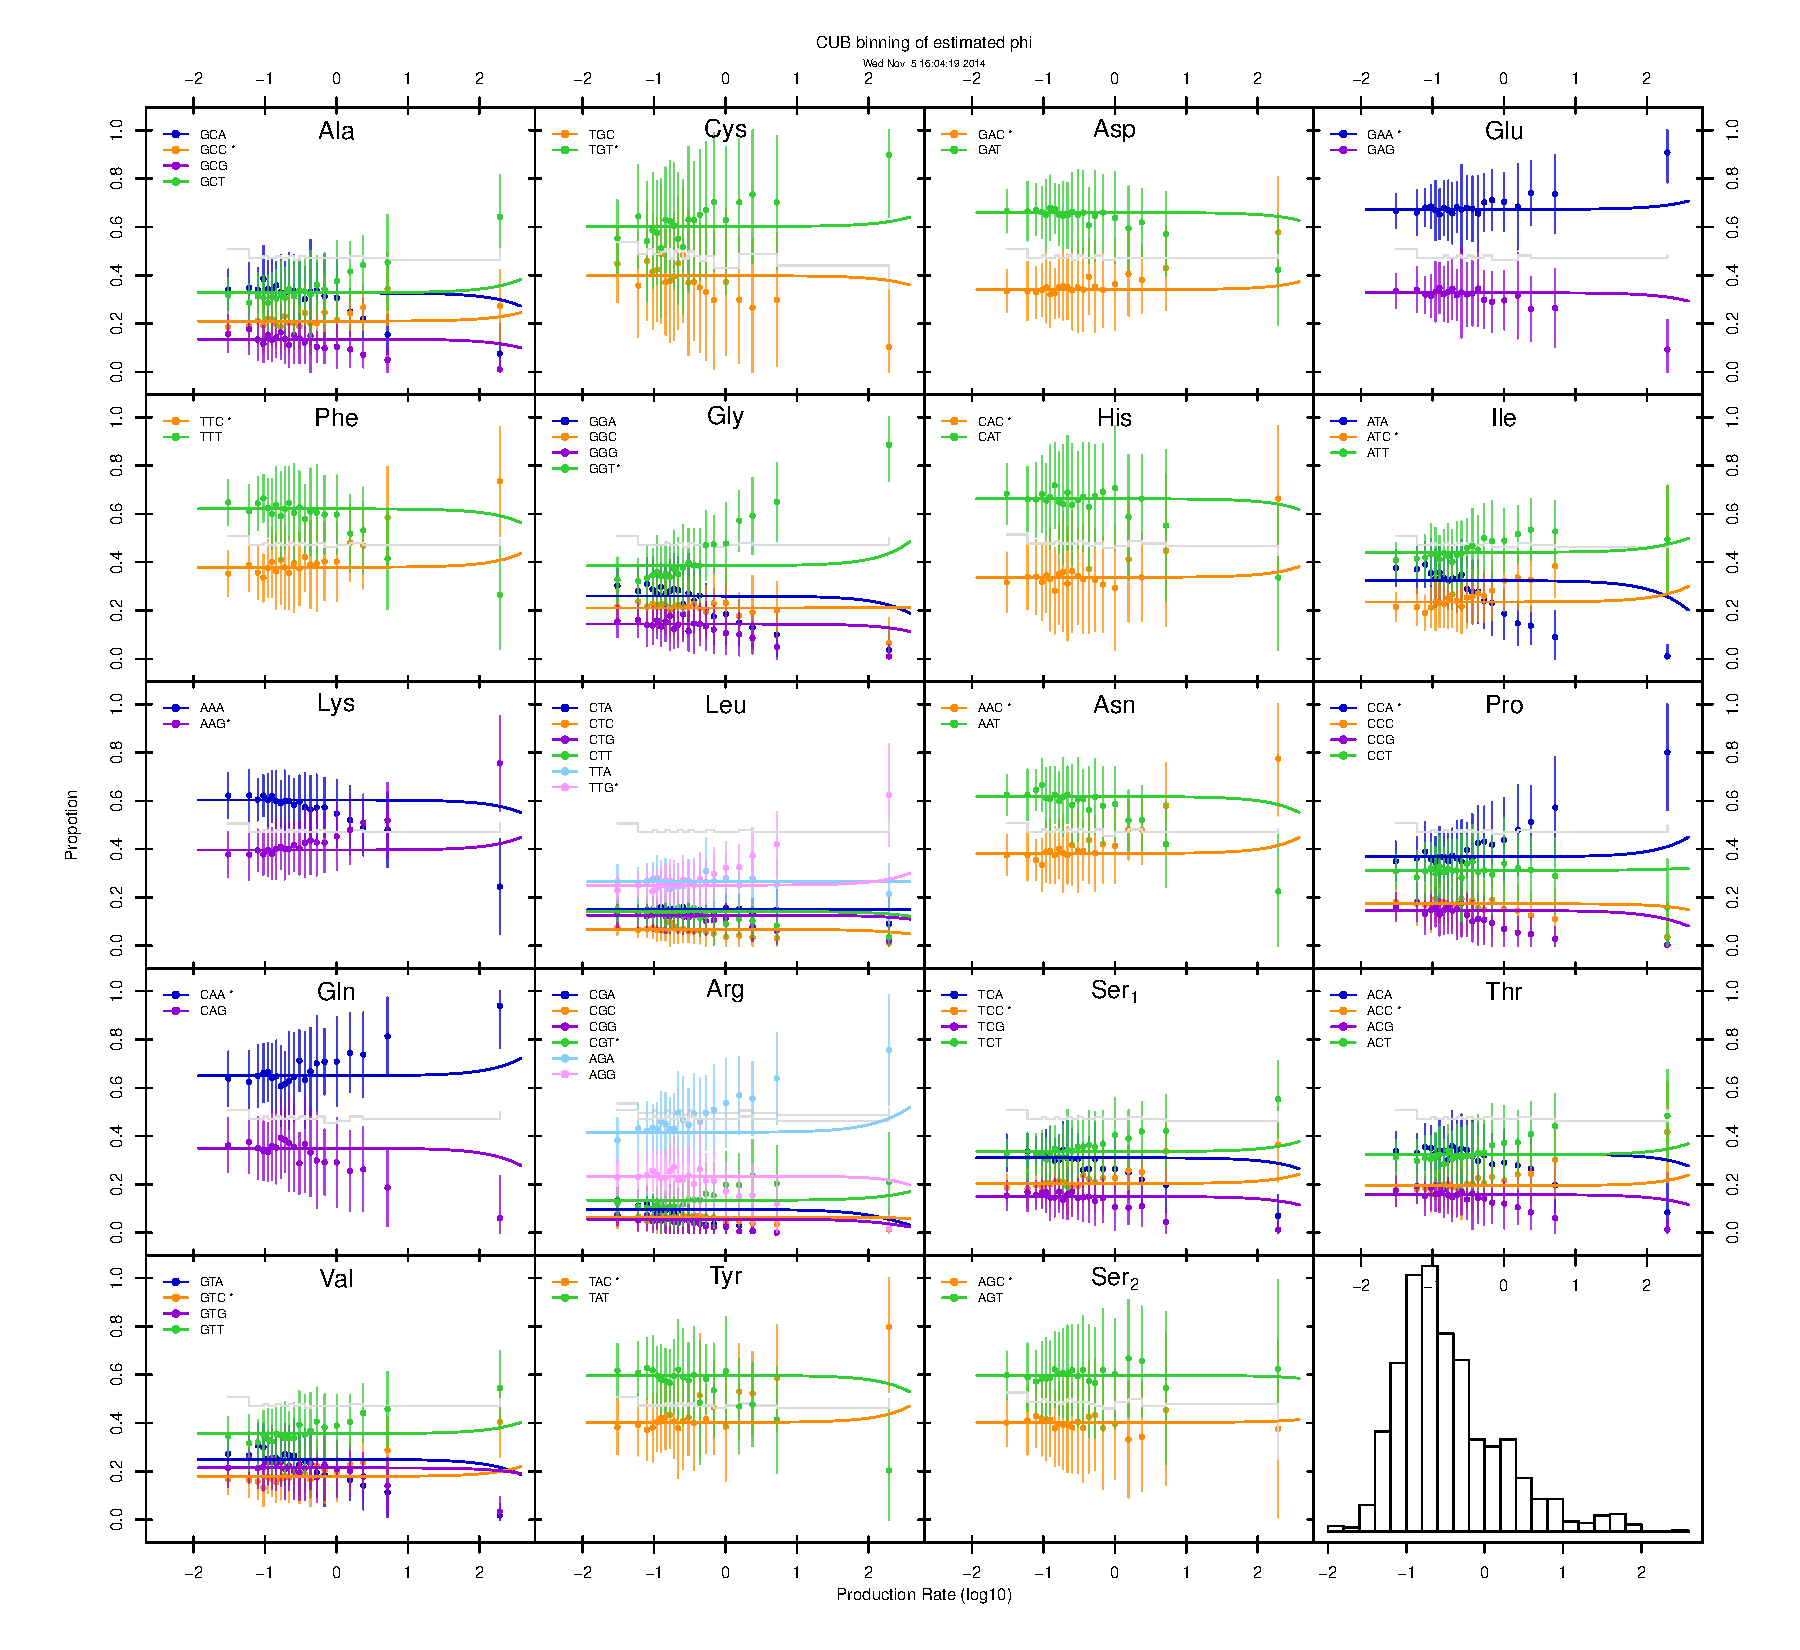
\includepdf[pages={1}]{data/1105_CUB_est_bin_8core.pdf}
%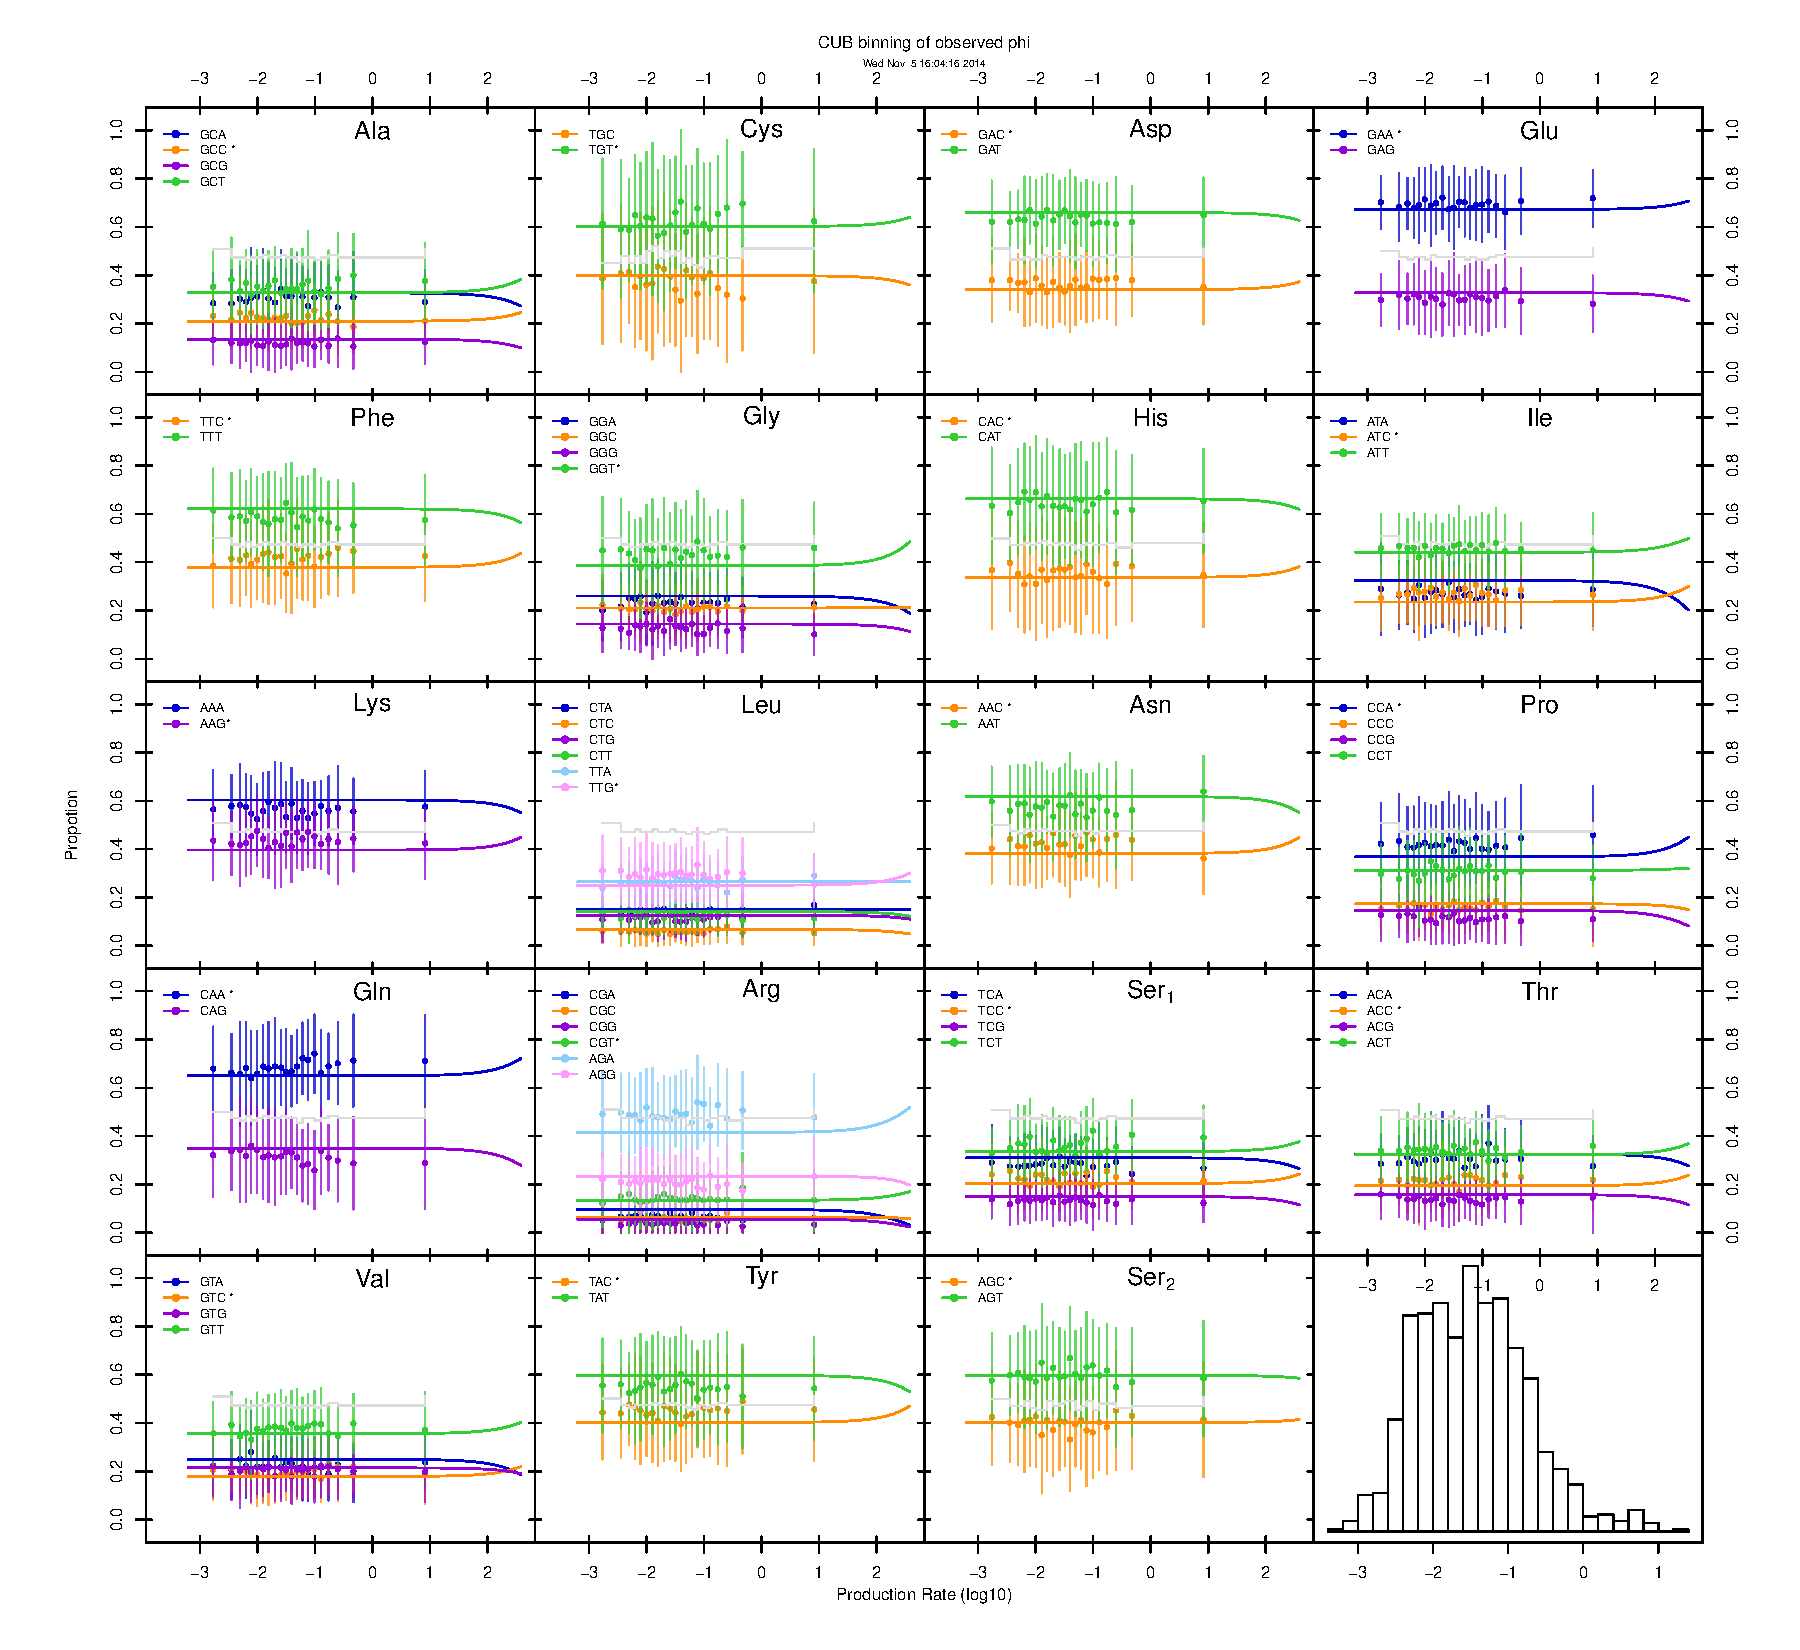
\includepdf[pages={1}]{data/1105_CUB_obs_bin_8core.pdf}
%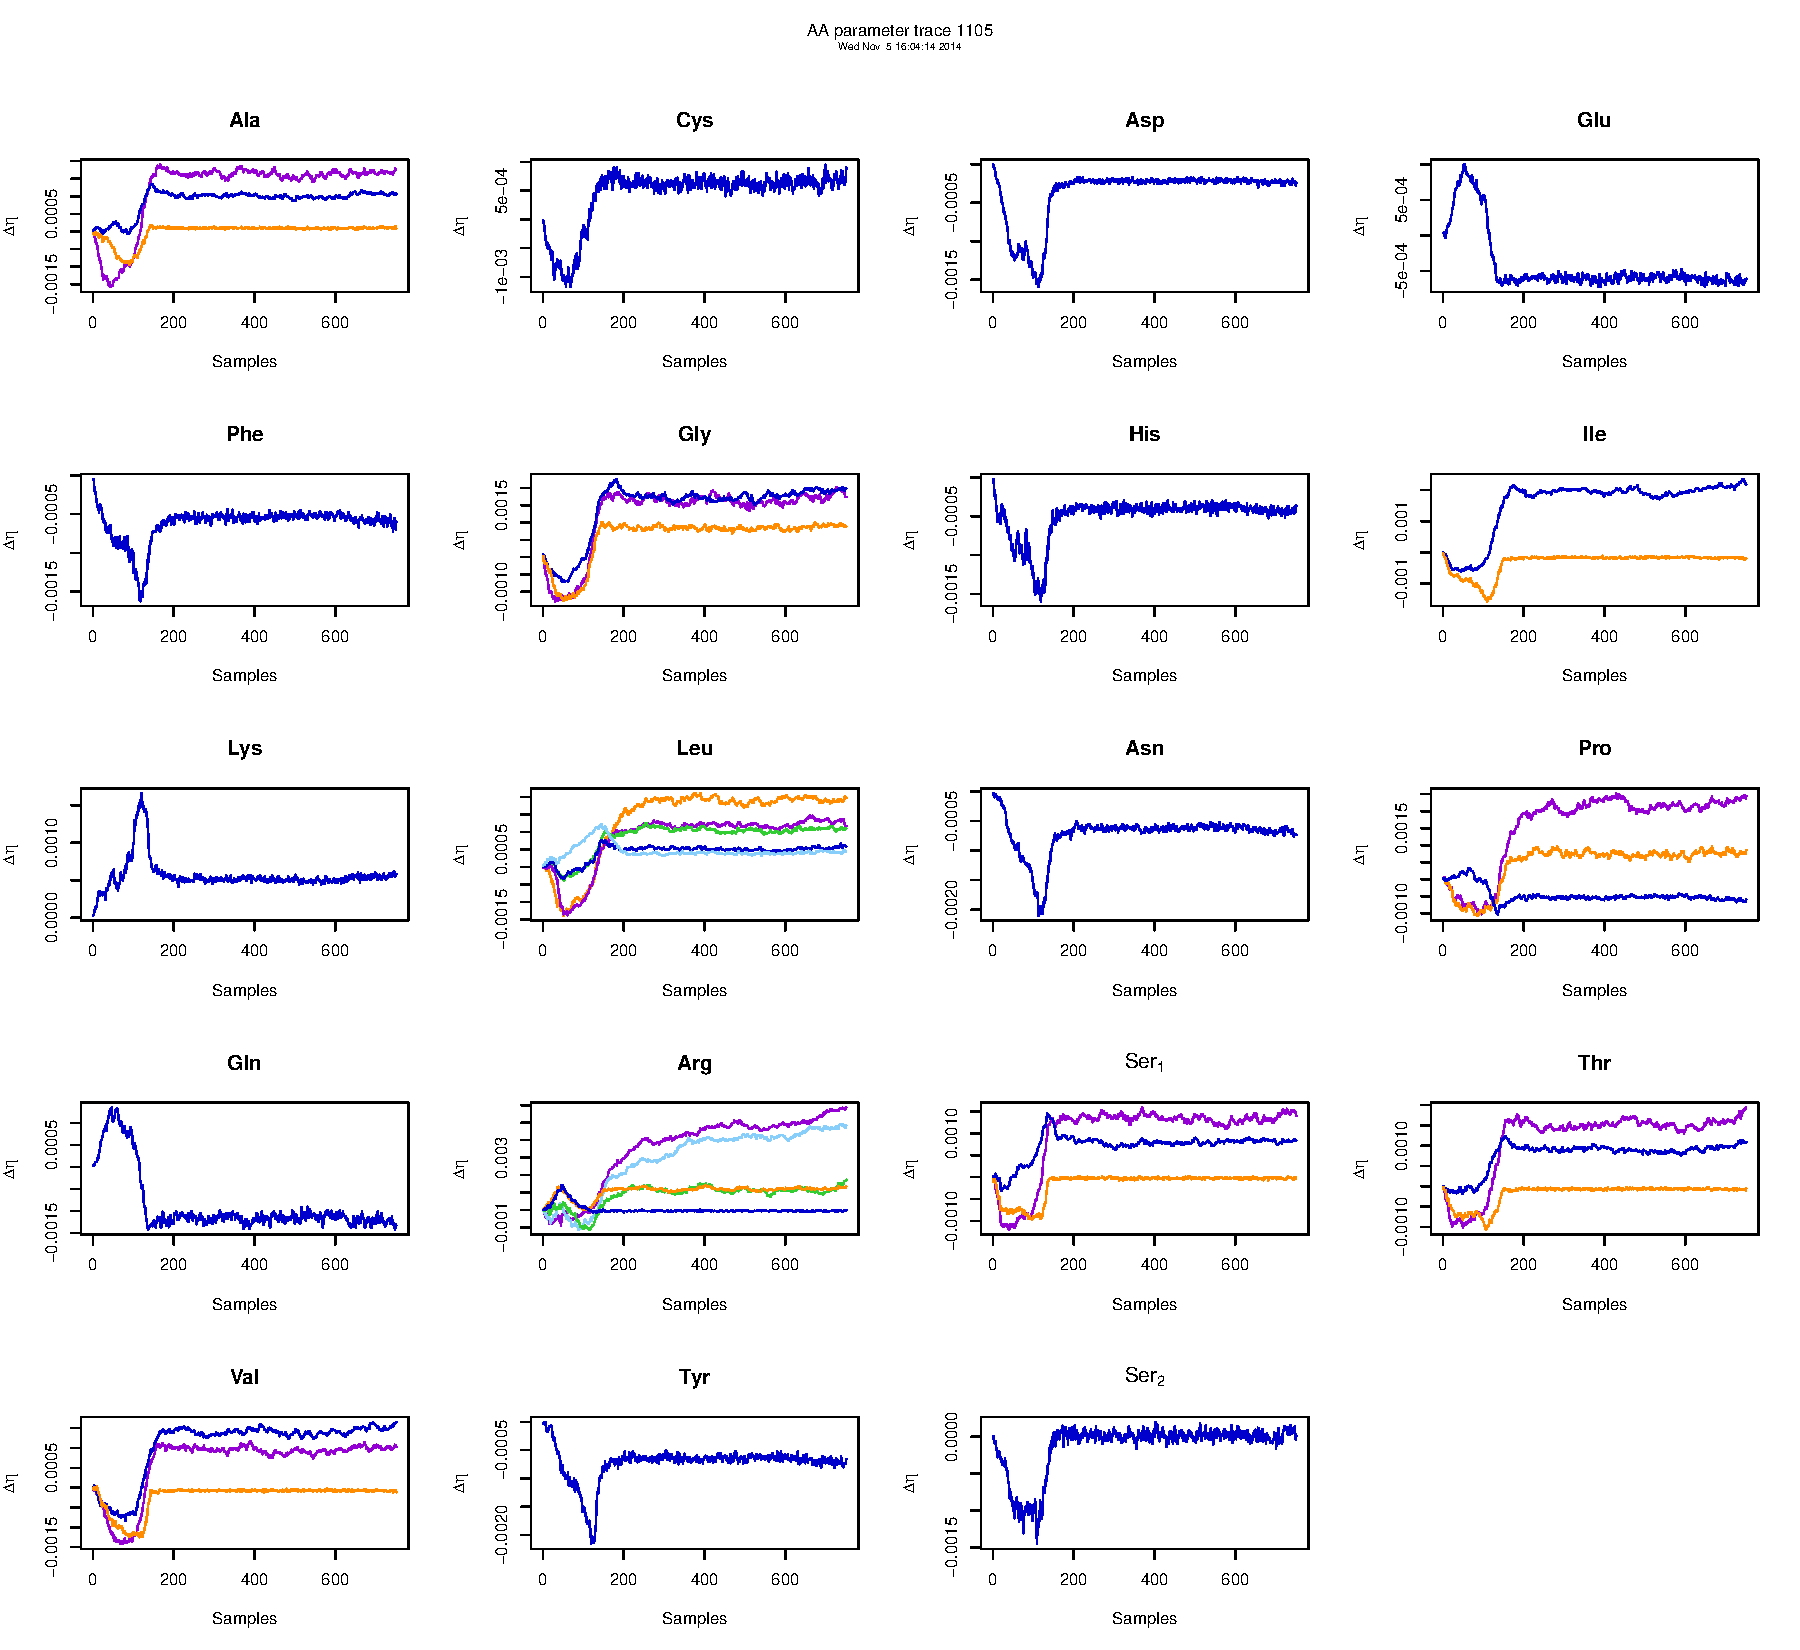
\includepdf[pages={1}]{data/1105_deltaeta_8core.pdf}
%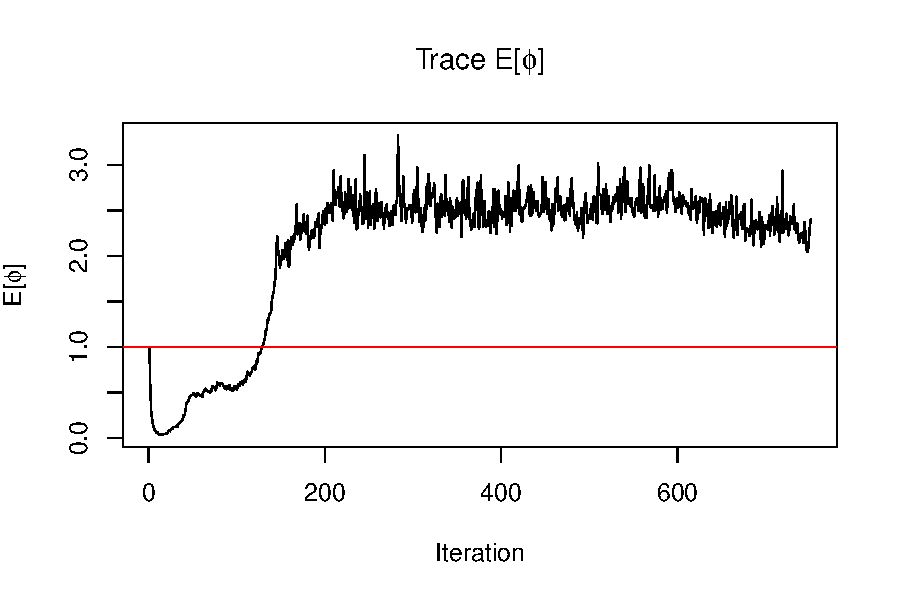
\includepdf[pages={1}]{data/1105_expPhi_trace_8core.pdf}
%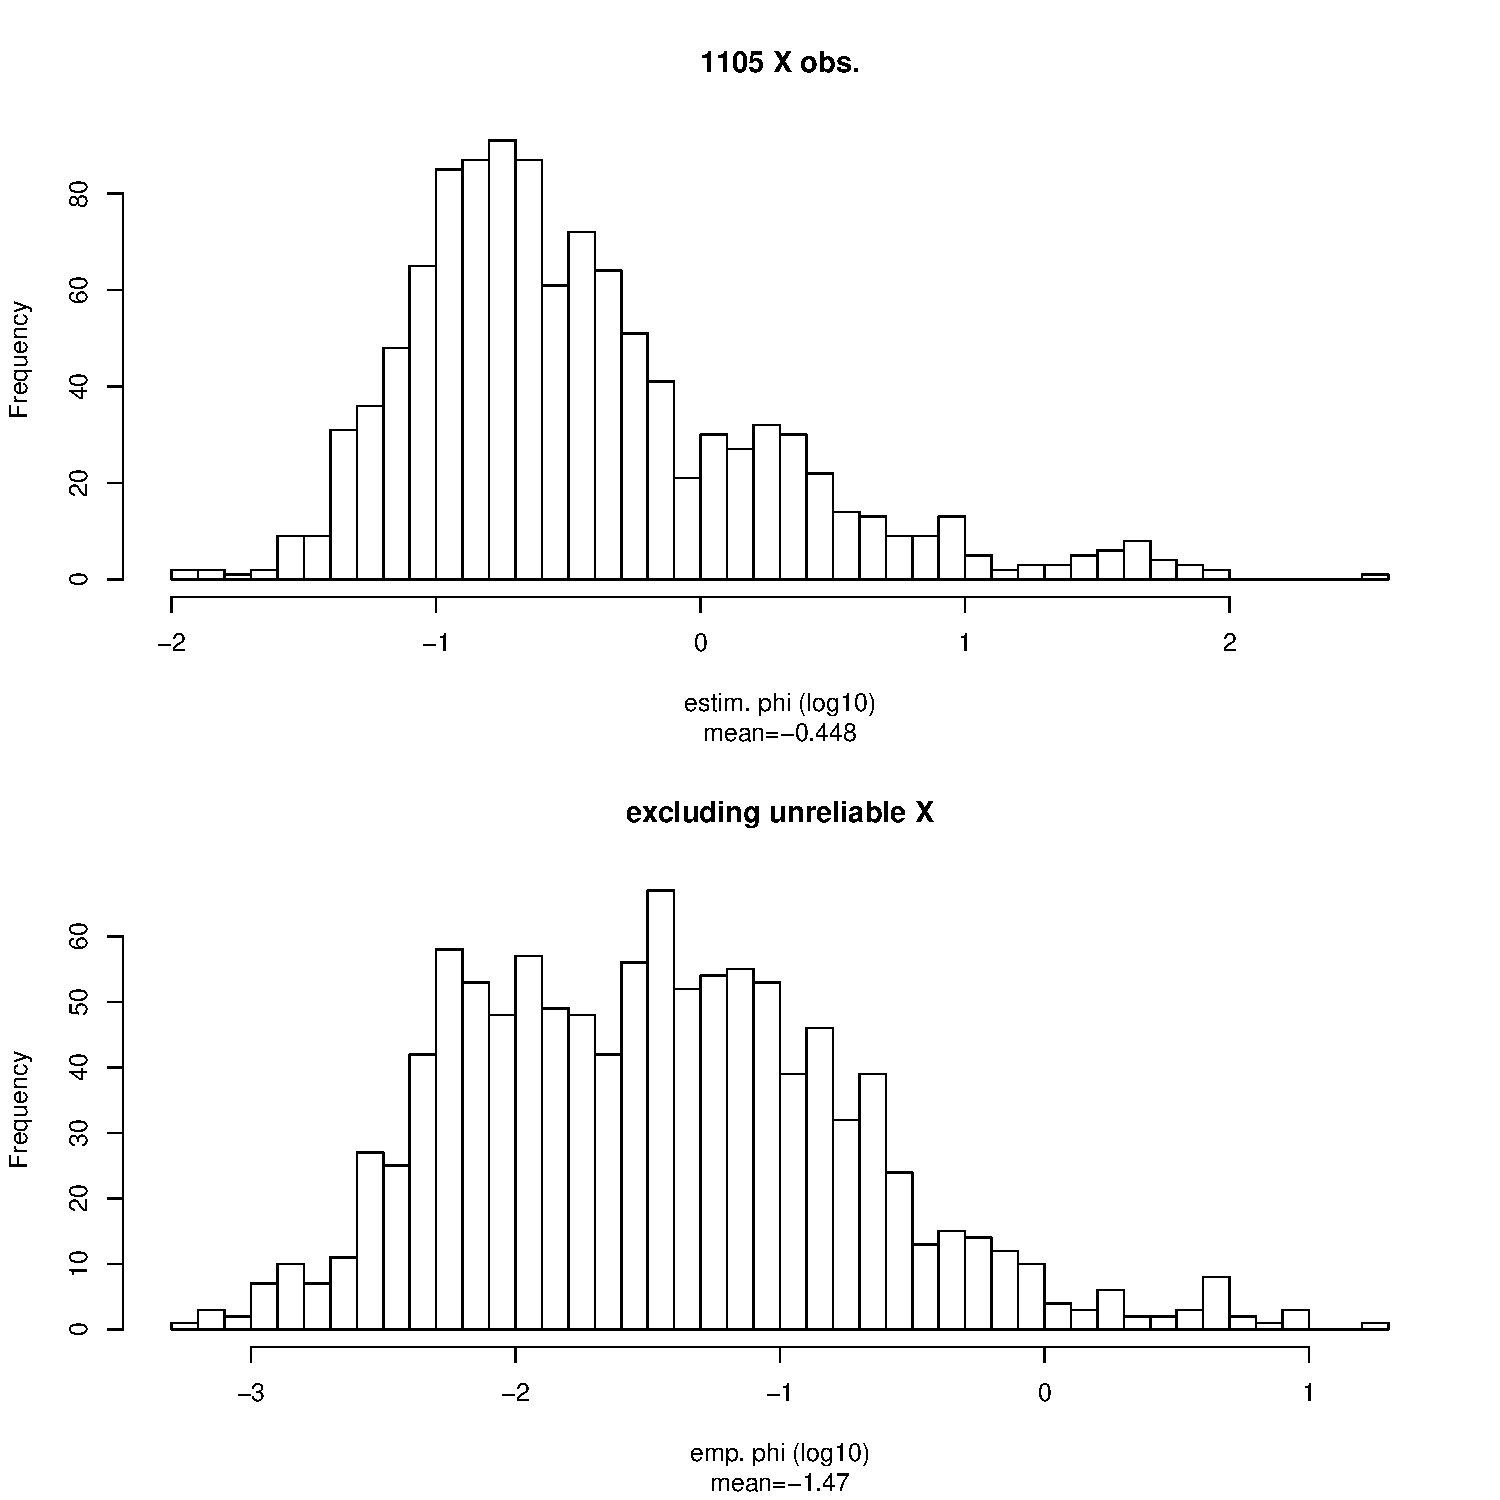
\includepdf[pages={1}]{data/1105_histogram_8core.pdf}
%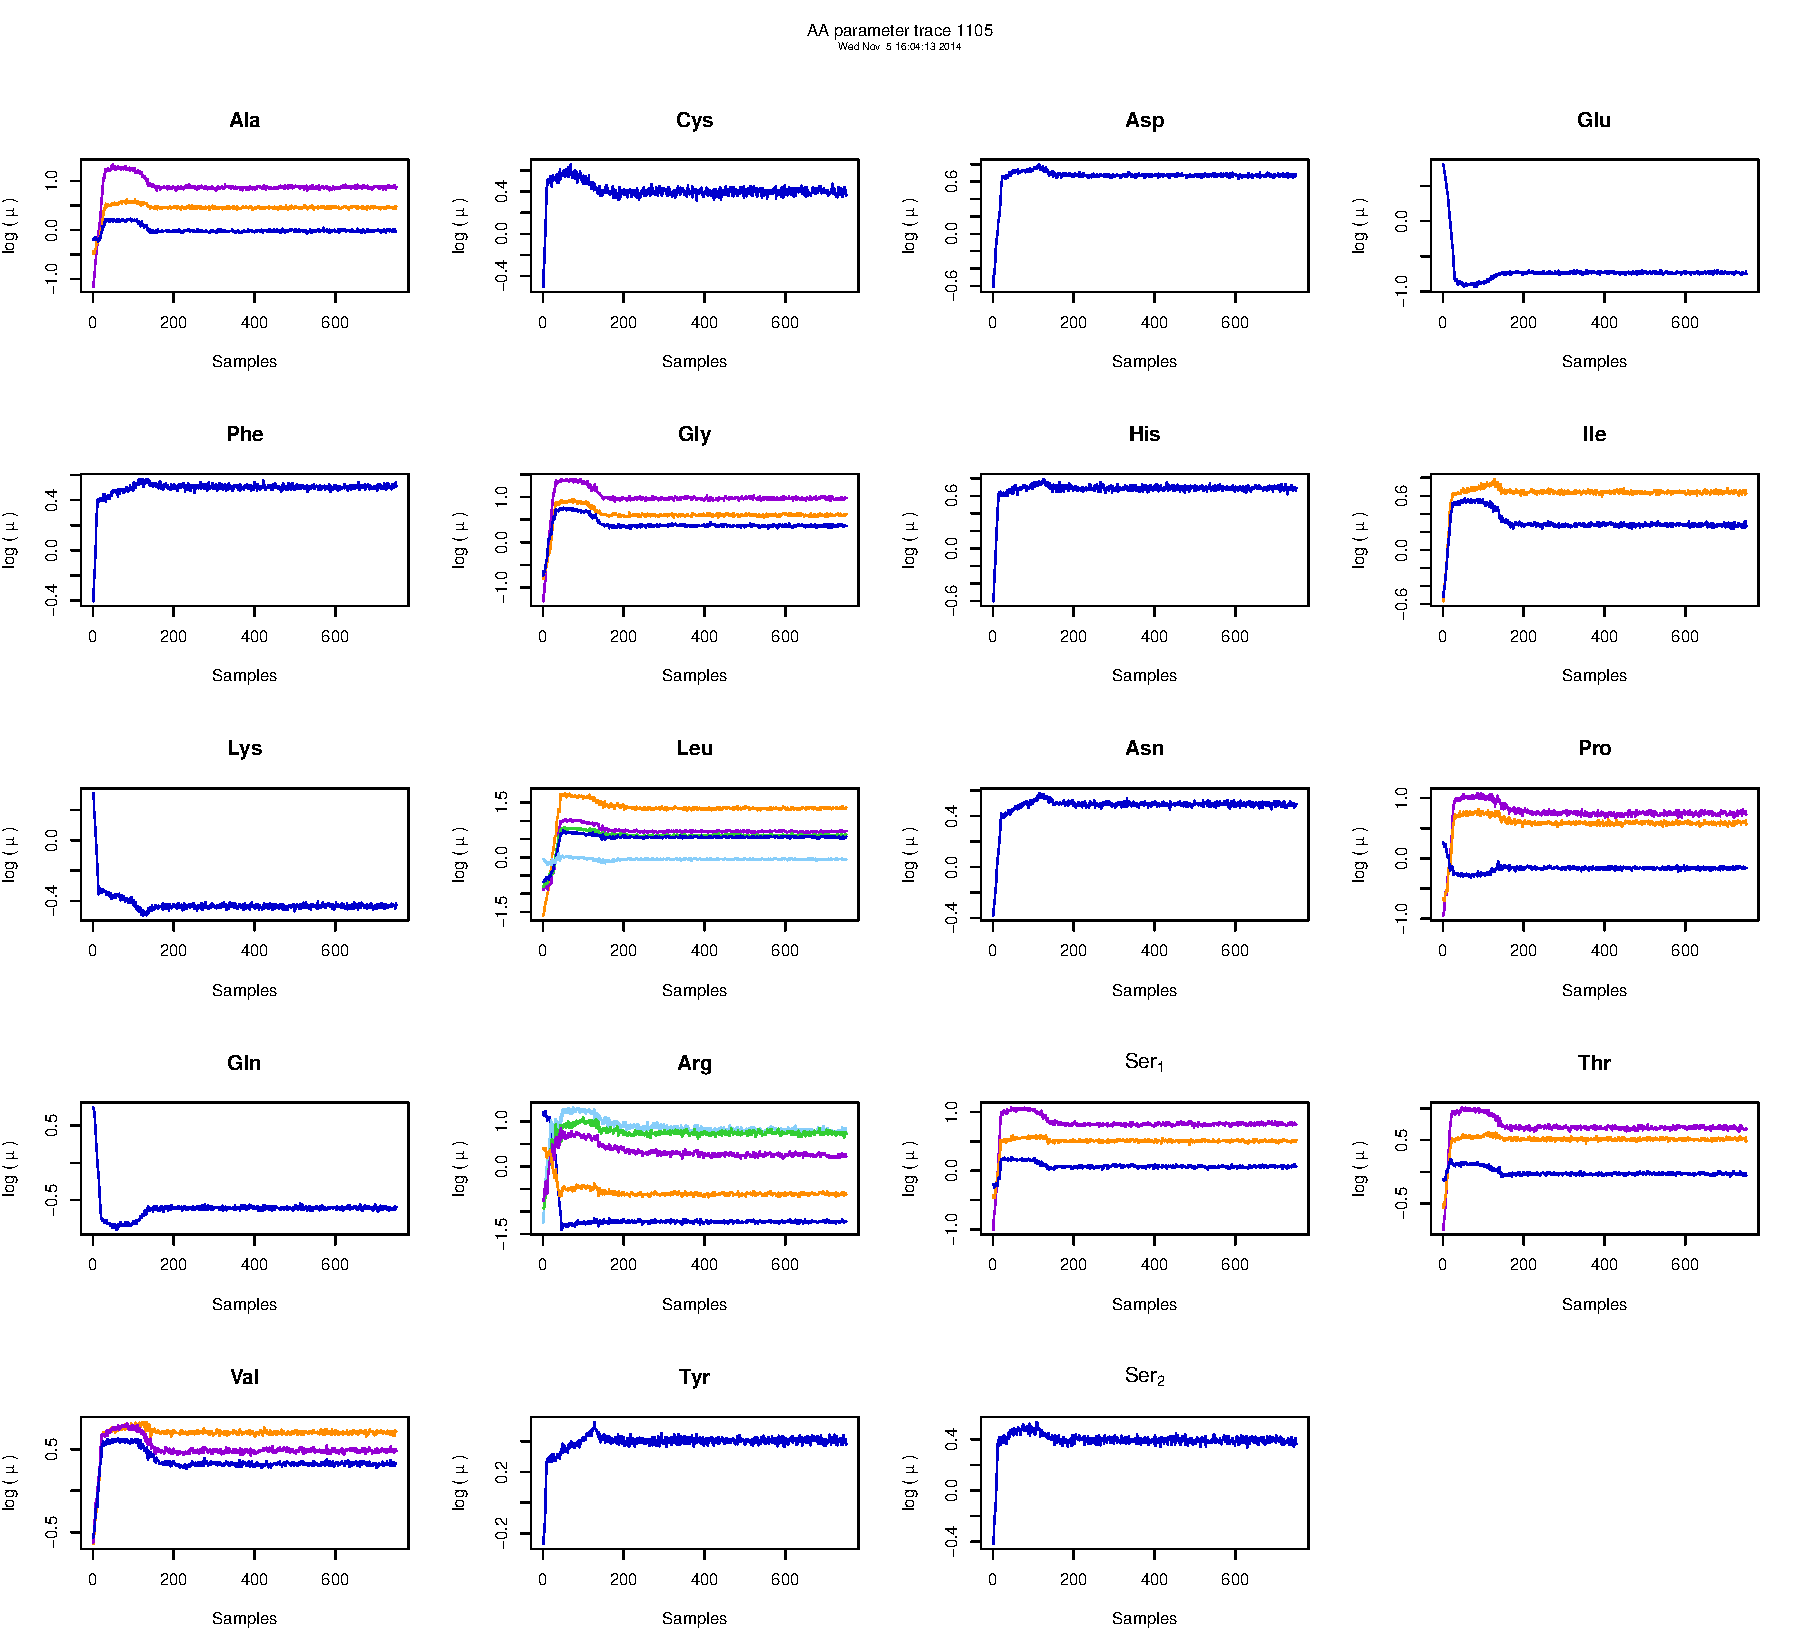
\includepdf[pages={1}]{data/1105_logmu_8core.pdf}
%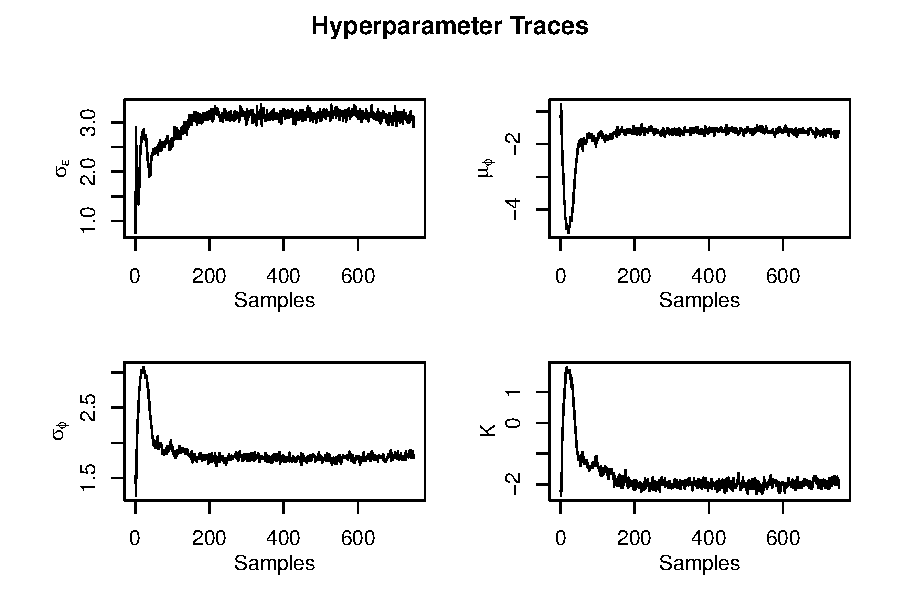
\includepdf[pages={1}]{data/1105_pMat_trace_8core.pdf}
%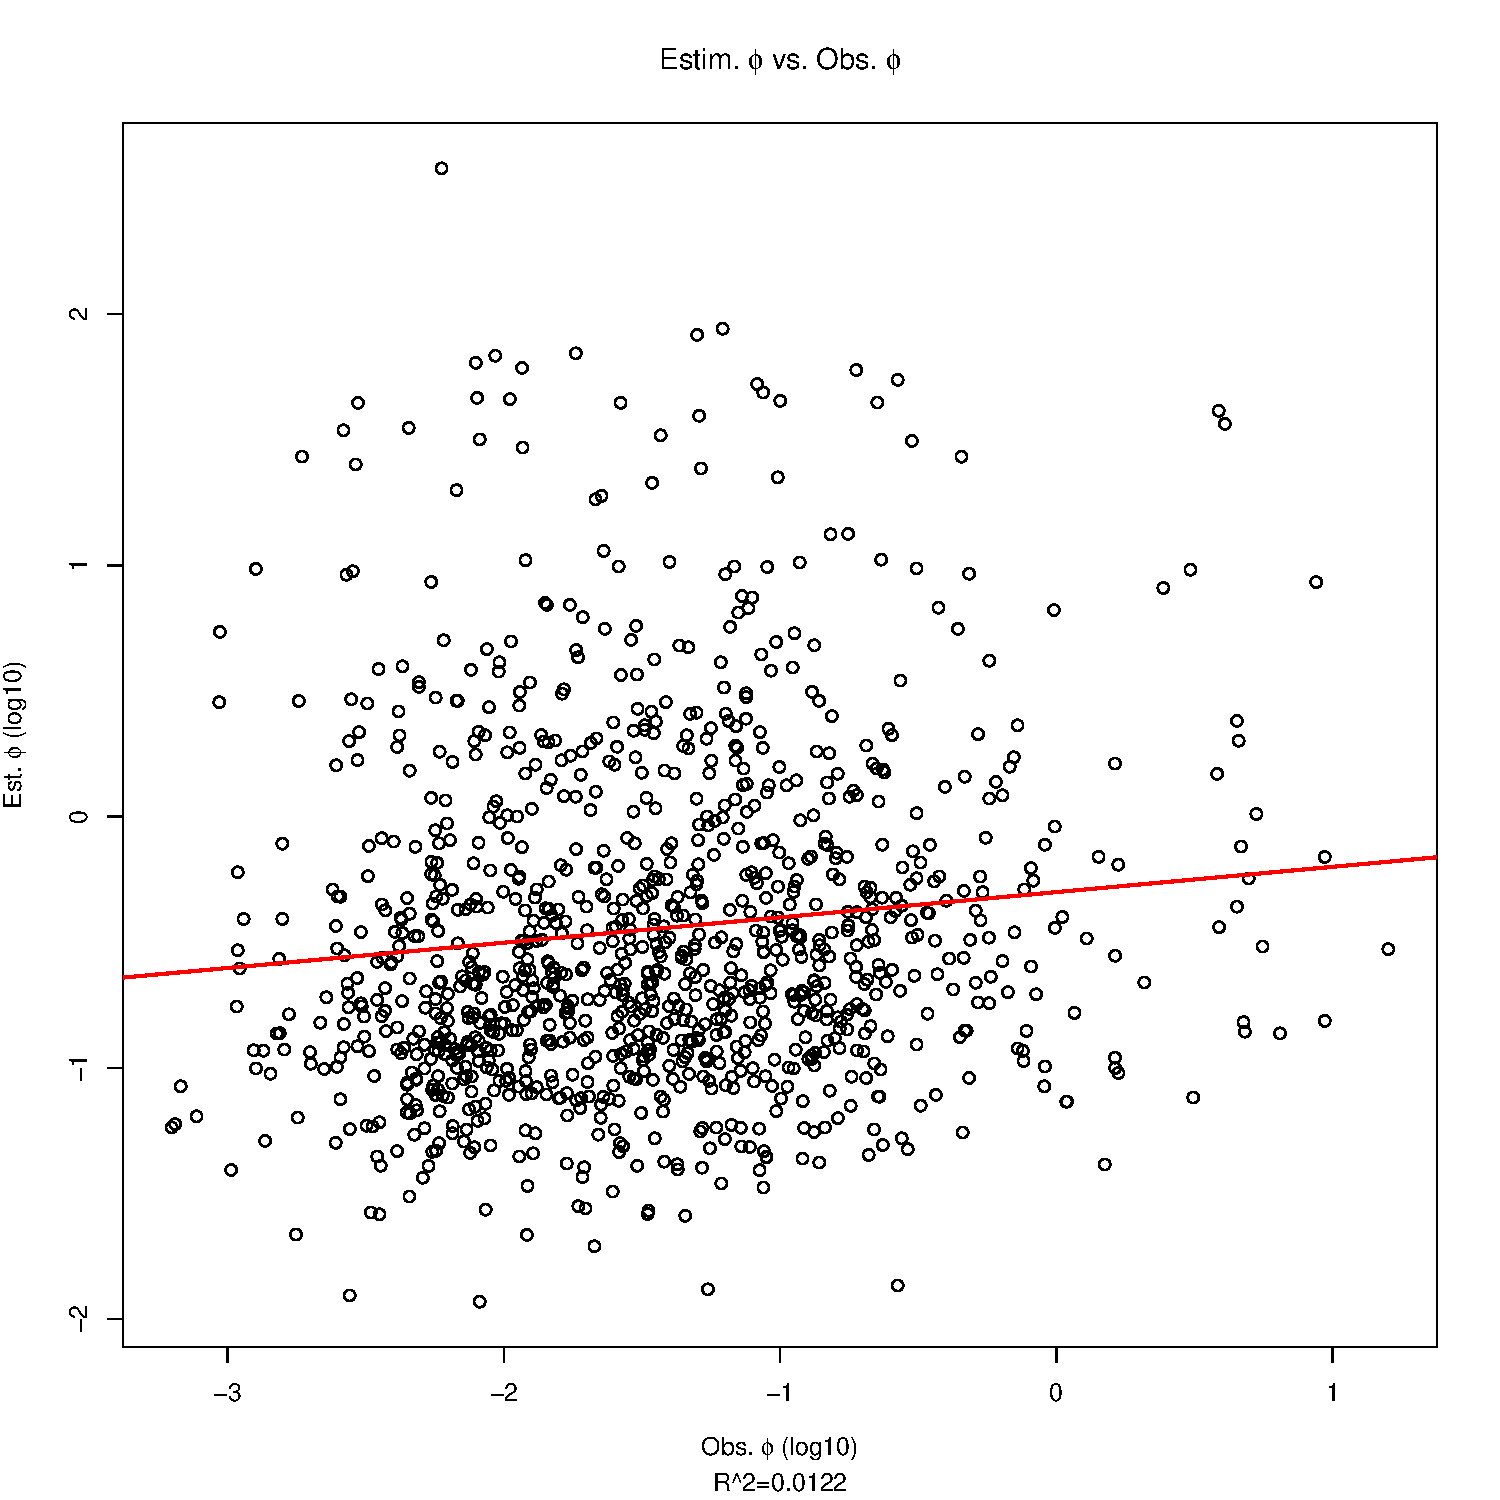
\includepdf[pages={1}]{data/1105_vs_obs_phi_8core.pdf}

\begin{verbatim}
{{ REMOVED FOR BREVITY. SEE data/1105*.pdf }}
\end{verbatim}


Note how different the $\Delta\omega$ values are between Preston's yeast genome and the REU students' yeast genome.

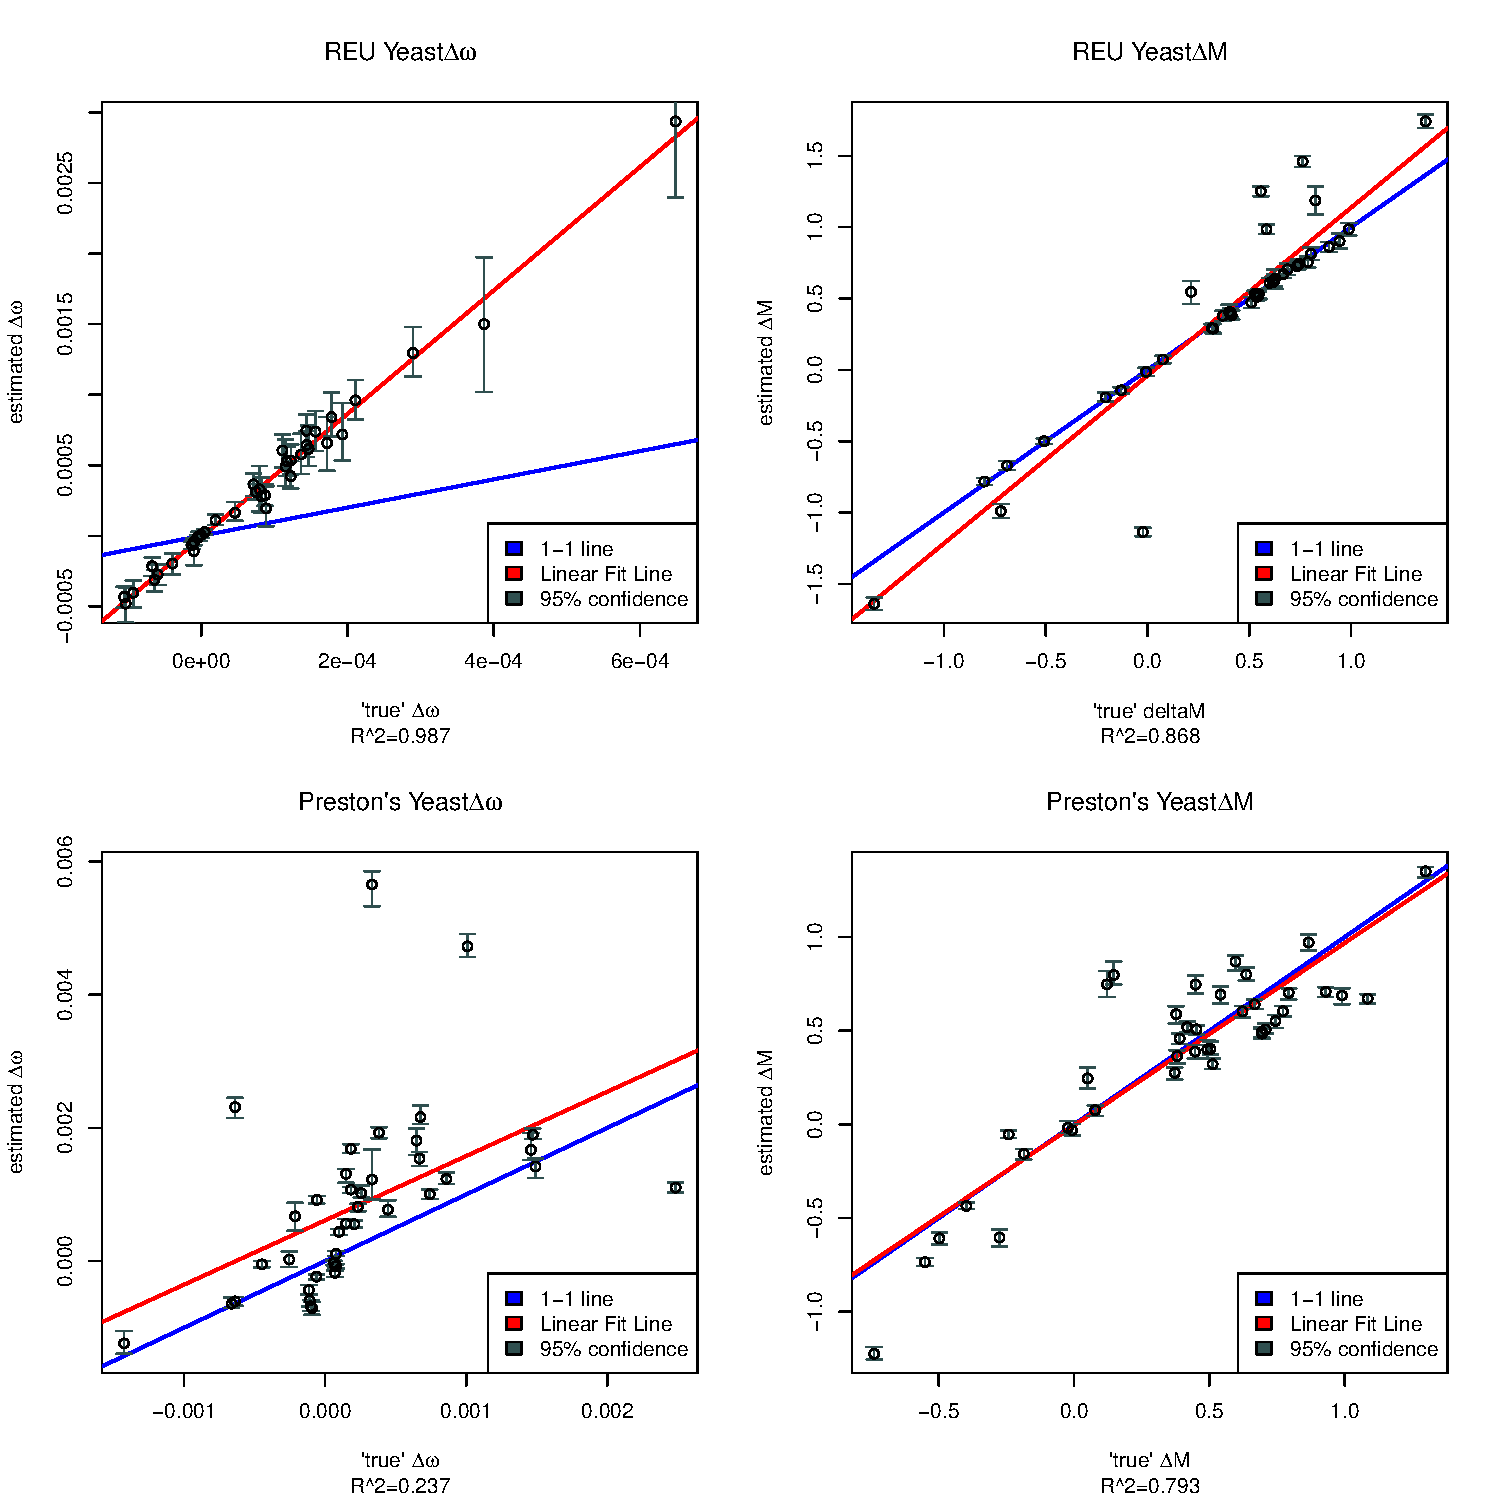
\includepdf[pages={1}]{data/1105_sidebyside.pdf}

\subsubsection{Longer Run?}

A longer run creates some interesting results. I did a run that used 7500 samples instead of 750 (which, since I'm thinning by 10, it's actually 75,000 proposals).

Here's the results (Large run is on the left, small run is on the right)

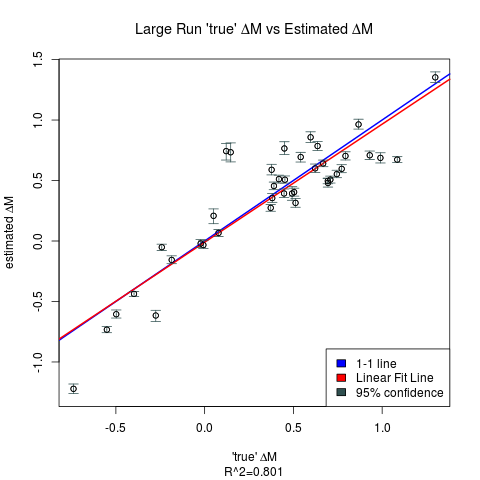
\includegraphics[width=0.5\textwidth]{data/mu_largerun.png}
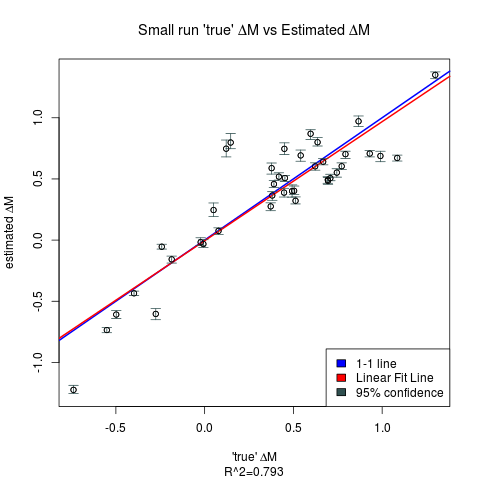
\includegraphics[width=0.5\textwidth]{data/mu_smallrun.png}

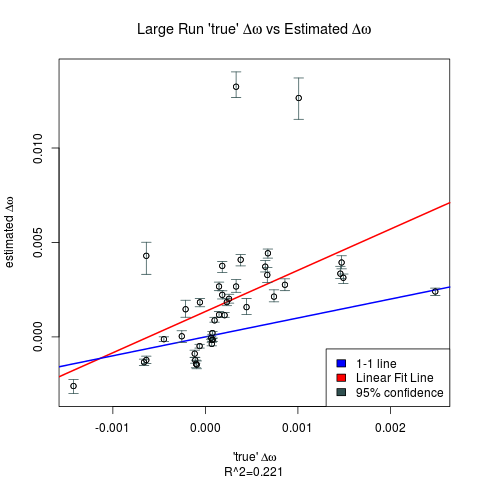
\includegraphics[width=0.5\textwidth]{data/omega_largerun.png}
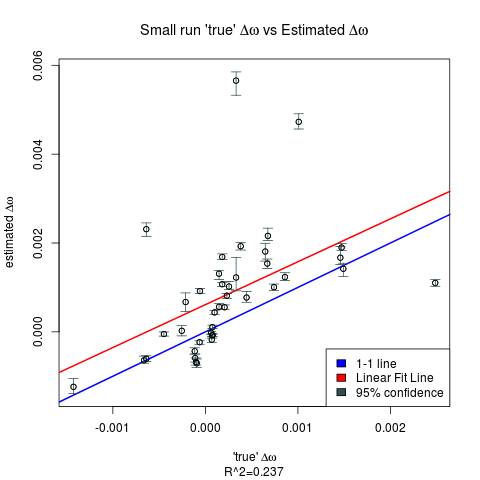
\includegraphics[width=0.5\textwidth]{data/omega_smallrun.png}

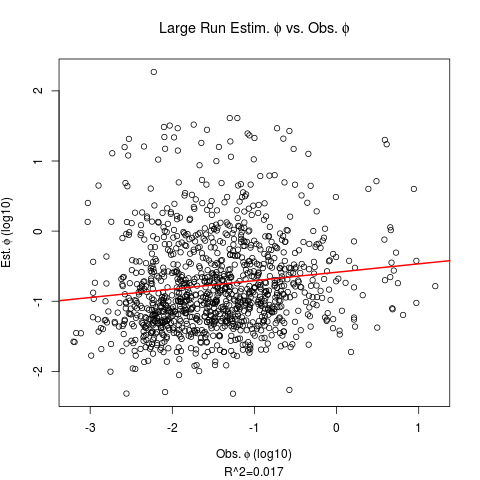
\includegraphics[width=0.5\textwidth]{data/phi_largerun.png}
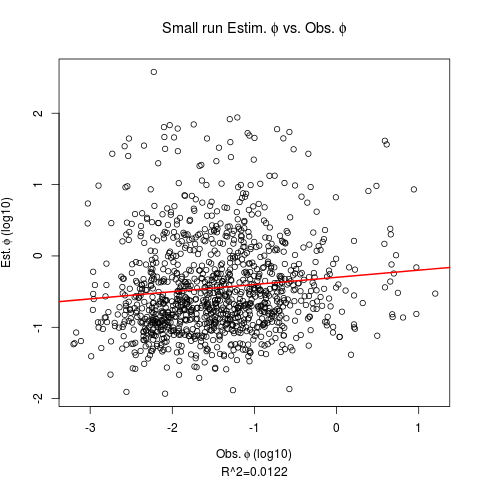
\includegraphics[width=0.5\textwidth]{data/phi_smallrun.png}

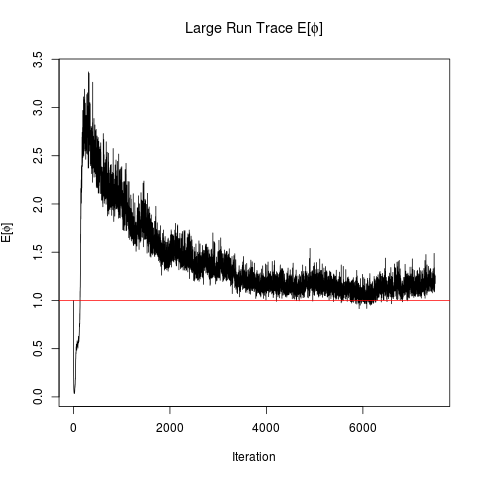
\includegraphics[width=0.5\textwidth]{data/ephi_largerun.png}
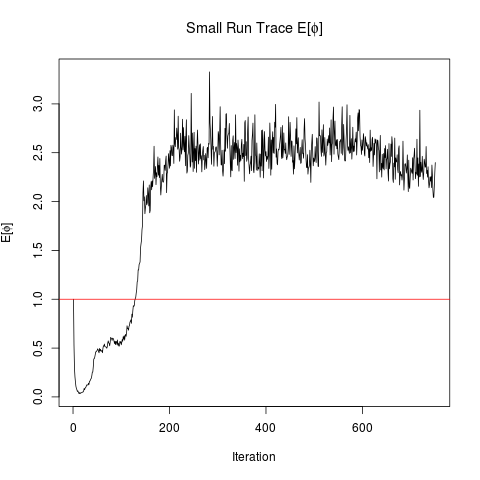
\includegraphics[width=0.5\textwidth]{data/ephi_smallrun.png}

The most relevant thing in my opinion is the E($\phi$) graphs. E($\phi$) should hover around 1. in the small run, it leapt up to 3, and I was concerned this was an inherent problem in the code. But it appears that the model simply hadn't converged.

\subsection{Other Genomes}

\subsubsection{Entire Preston's Yeast}

I fixed an error in the visualize.r results by using the entire genome as the input, and letting the visualize function sort out what values belonged to who. This caused my $R^2$ value to jump from .02 to .5, a huge improvement.

Because of this, I'm doing a cubfits run with the entire preston's yeast genome, to see how that affecst the results.

\subsubsection{Brewer's Yeast}
The yeast genome used for the paper, the git repository is 
\begin{verbatim}
/export/home/semppr/gitrepos/wcchen/logistic_analysis.git/
\end{verbatim}

The exported files can be found in 

\begin{verbatim}
/home/lbrown/logistic_analysis/p01-paper
\end{verbatim}

What follows is a comparison of 

\begin{enumerate}
\item A run of a random selection of 1/5th of the genes from the REU simulated yeast
\item A run of a random selection of 1/5th of the genes from Preston's simulated yeast
\item A run of Preston's entire simulated yeast genome
\item A run of the brewer's yeast genome that was used for the 2014 paper
\end{enumerate}

First, it will have the $\phi$ value comparison, then the codon usage bias for the 'true' $\phi$ values, and finally the codon usage bias for the phi values generated by the model. Each run was done with $\delta a_{1,2}$=0 and $a_2$=4. Each run ran for 3000 samples with 10x thinning, or 30,000 total proposed values, except for the REU yeast which was 1000 samples, or 10,000 total proposed values. Other collections of runs were done with differing values of $\delta a_{1,2}$ and $a_2$, especially for the partial Preston's Yeast, but those runs are not included for brevity.

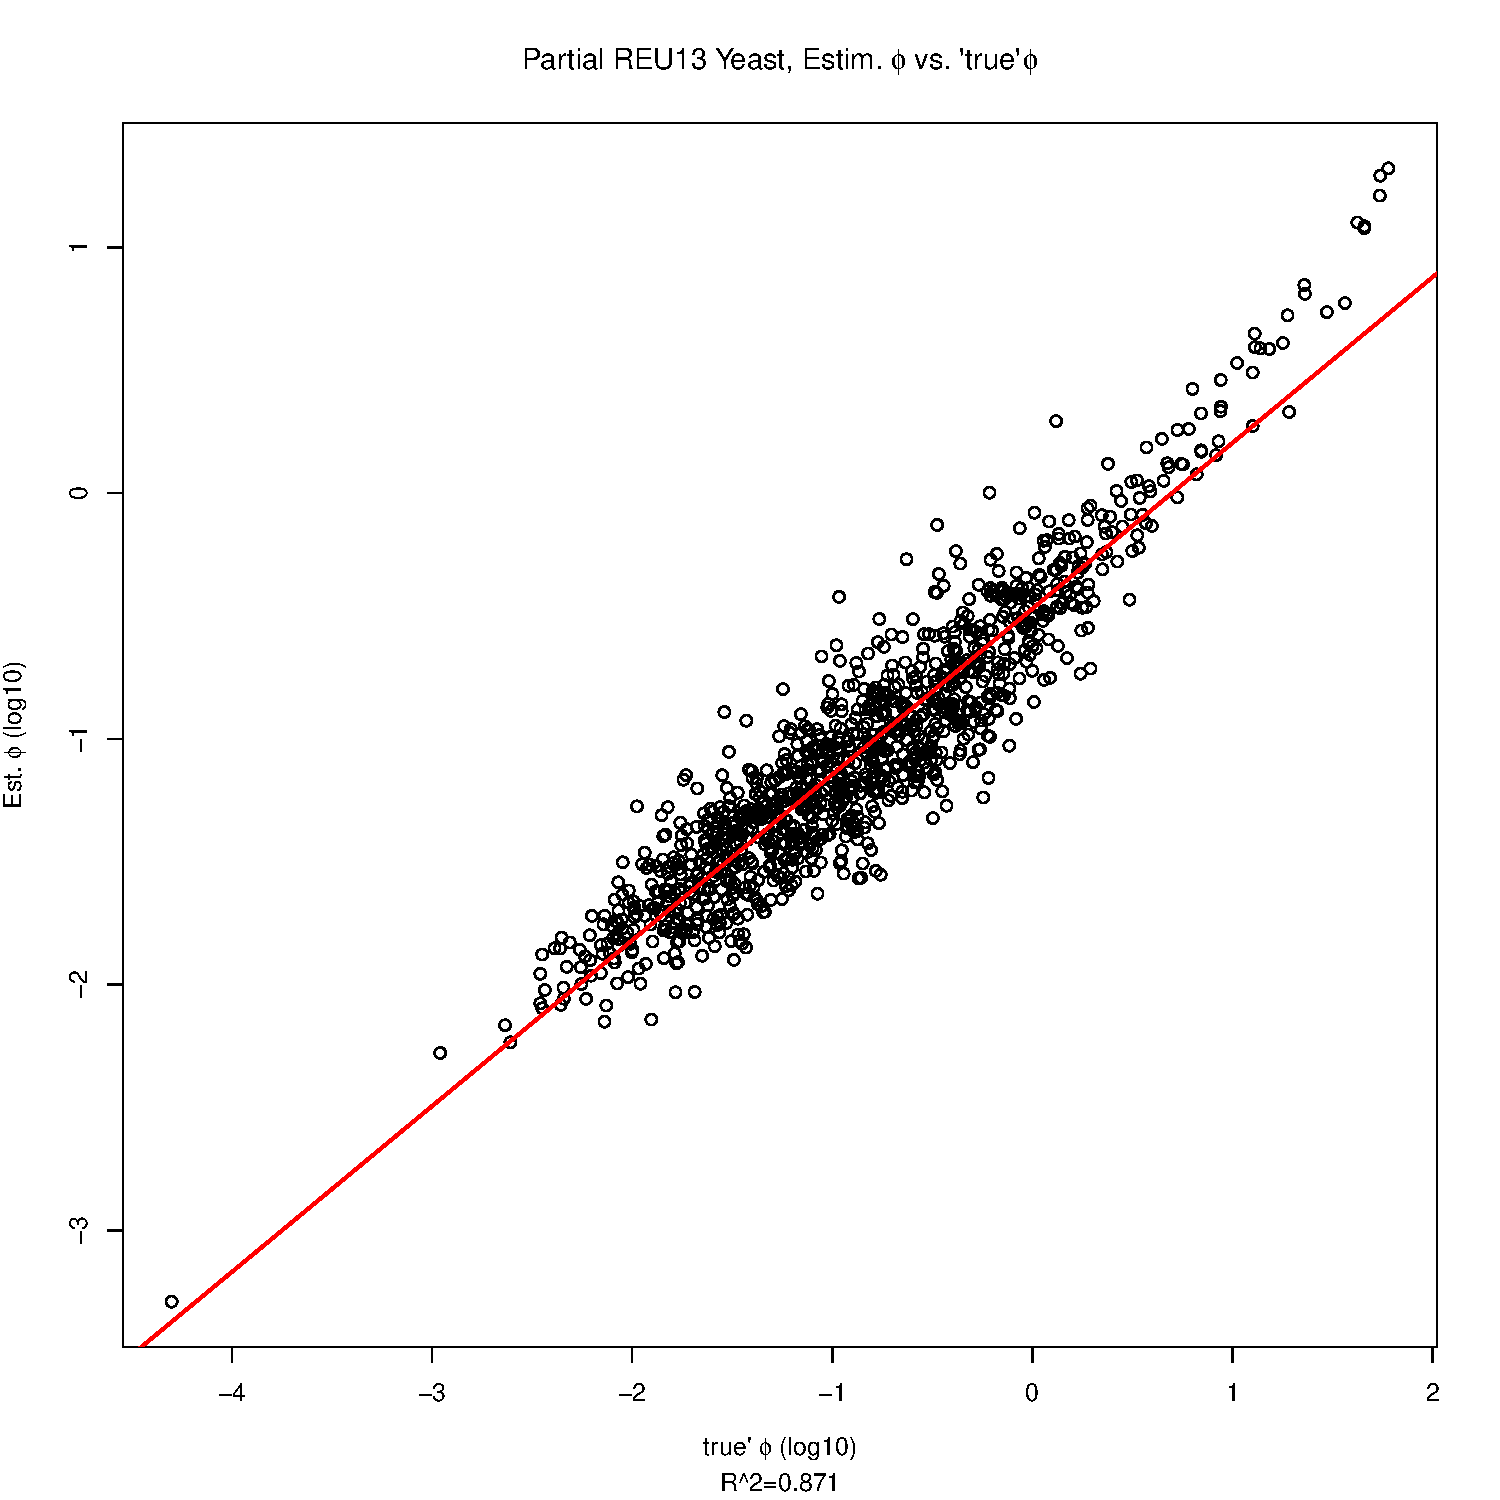
\includepdf[pages={1}]{data/partialREUYeast-Phi.pdf}
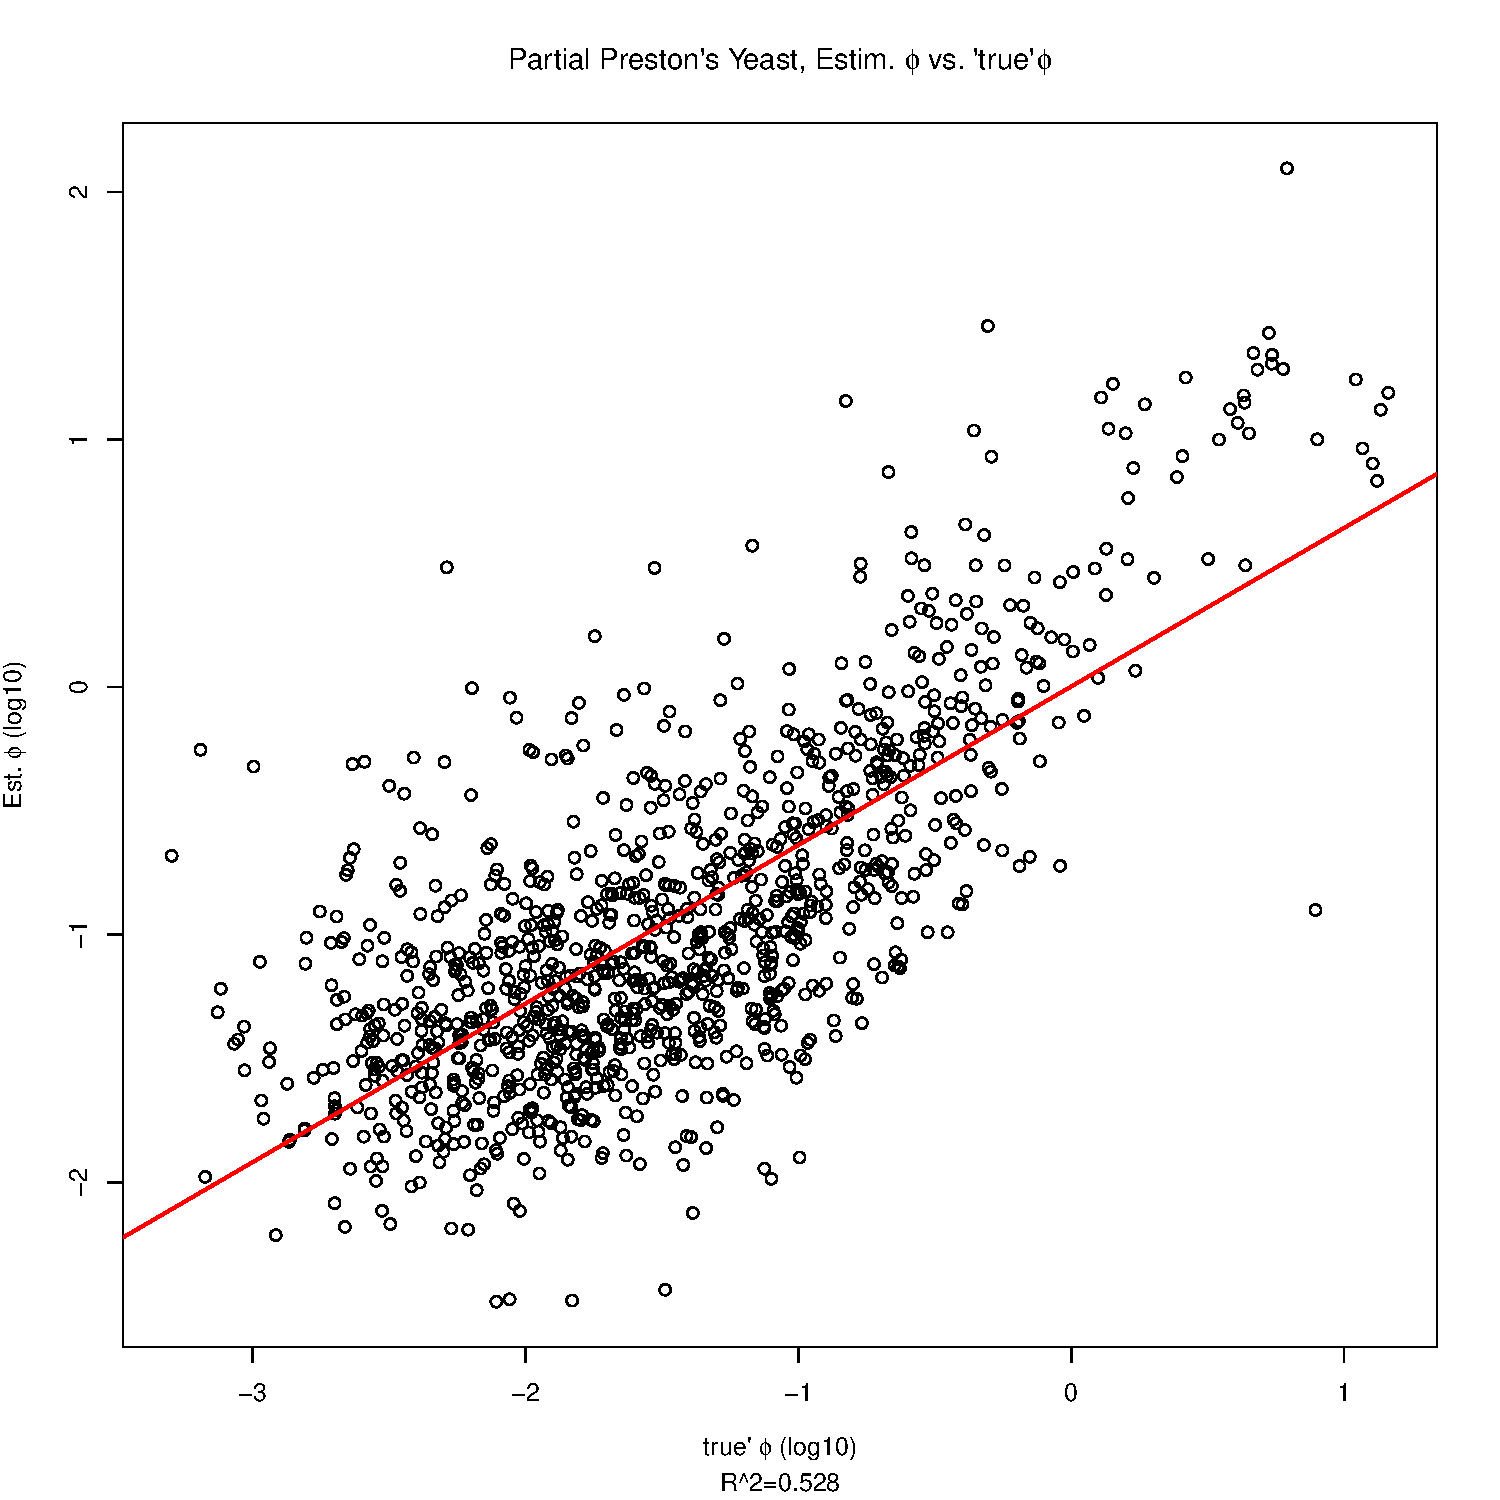
\includepdf[pages={1}]{data/partialPrestonYeast-Phi.pdf}
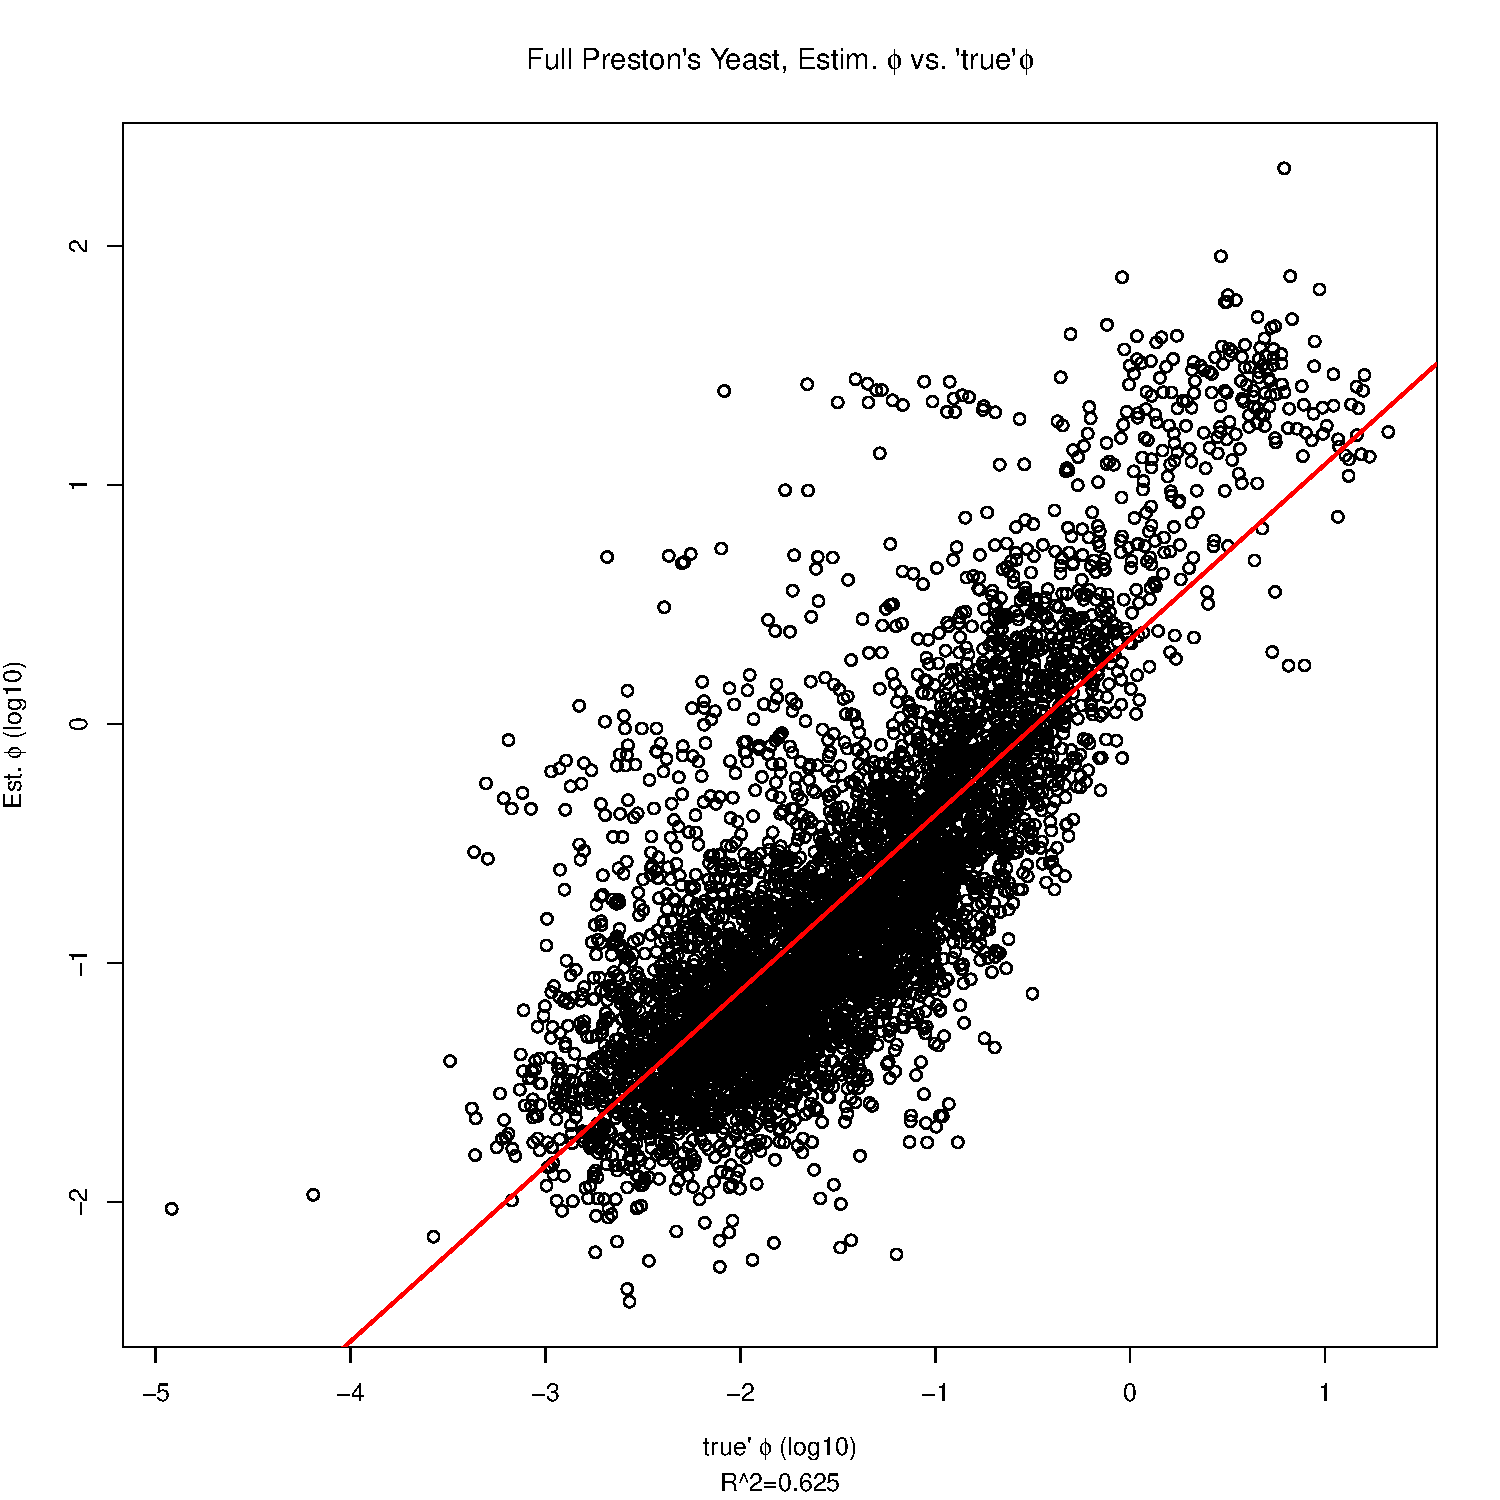
\includepdf[pages={1}]{data/fullPrestonYeast-Phi.pdf}
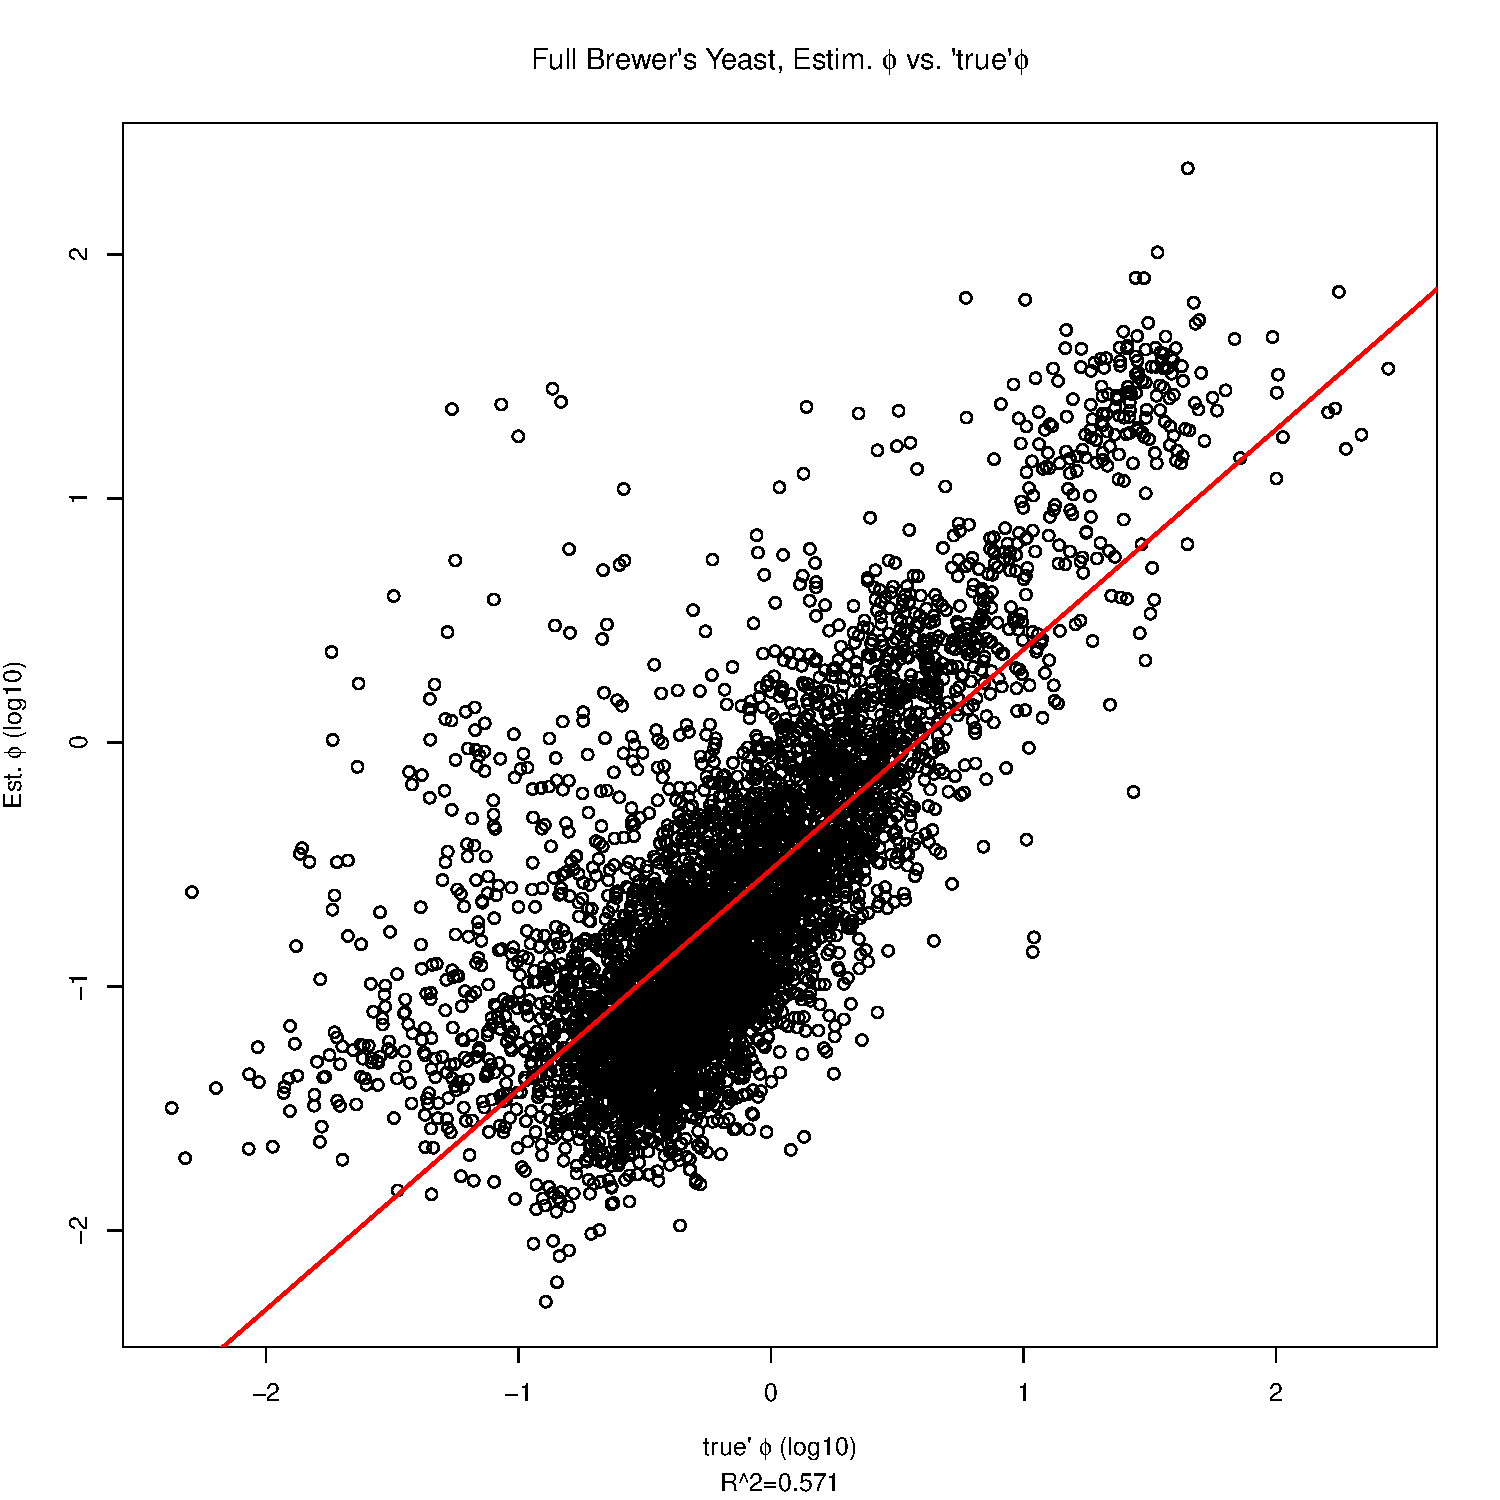
\includepdf[pages={1}]{data/fullBrewerYeast-Phi.pdf}

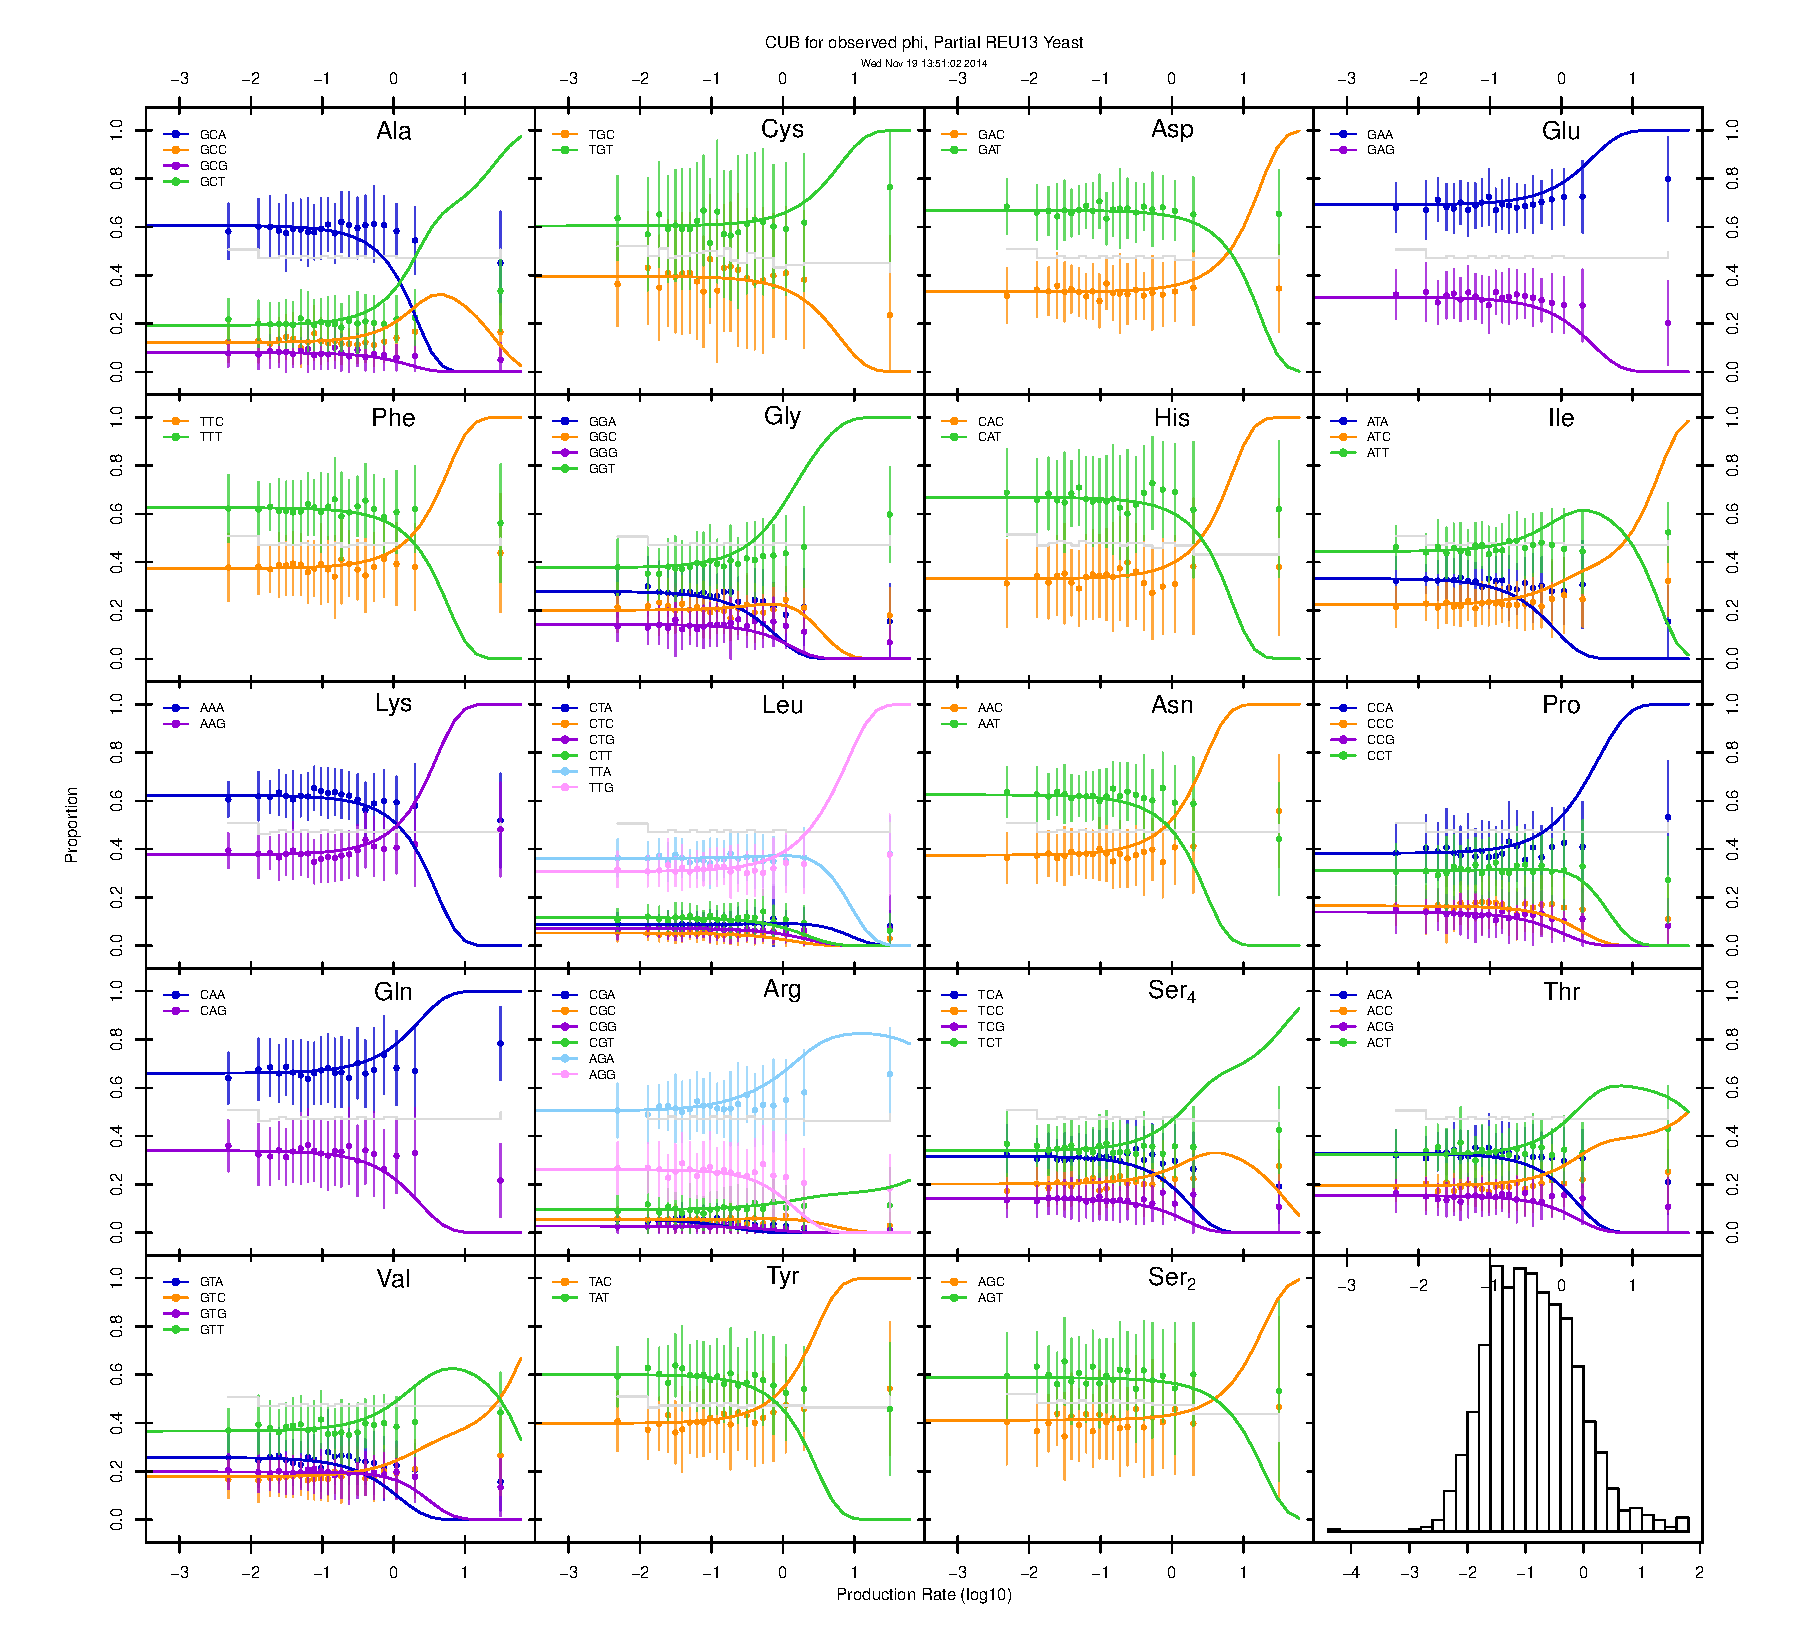
\includepdf[pages={1}]{data/partialREUYeast-CUBobsPhi.pdf}
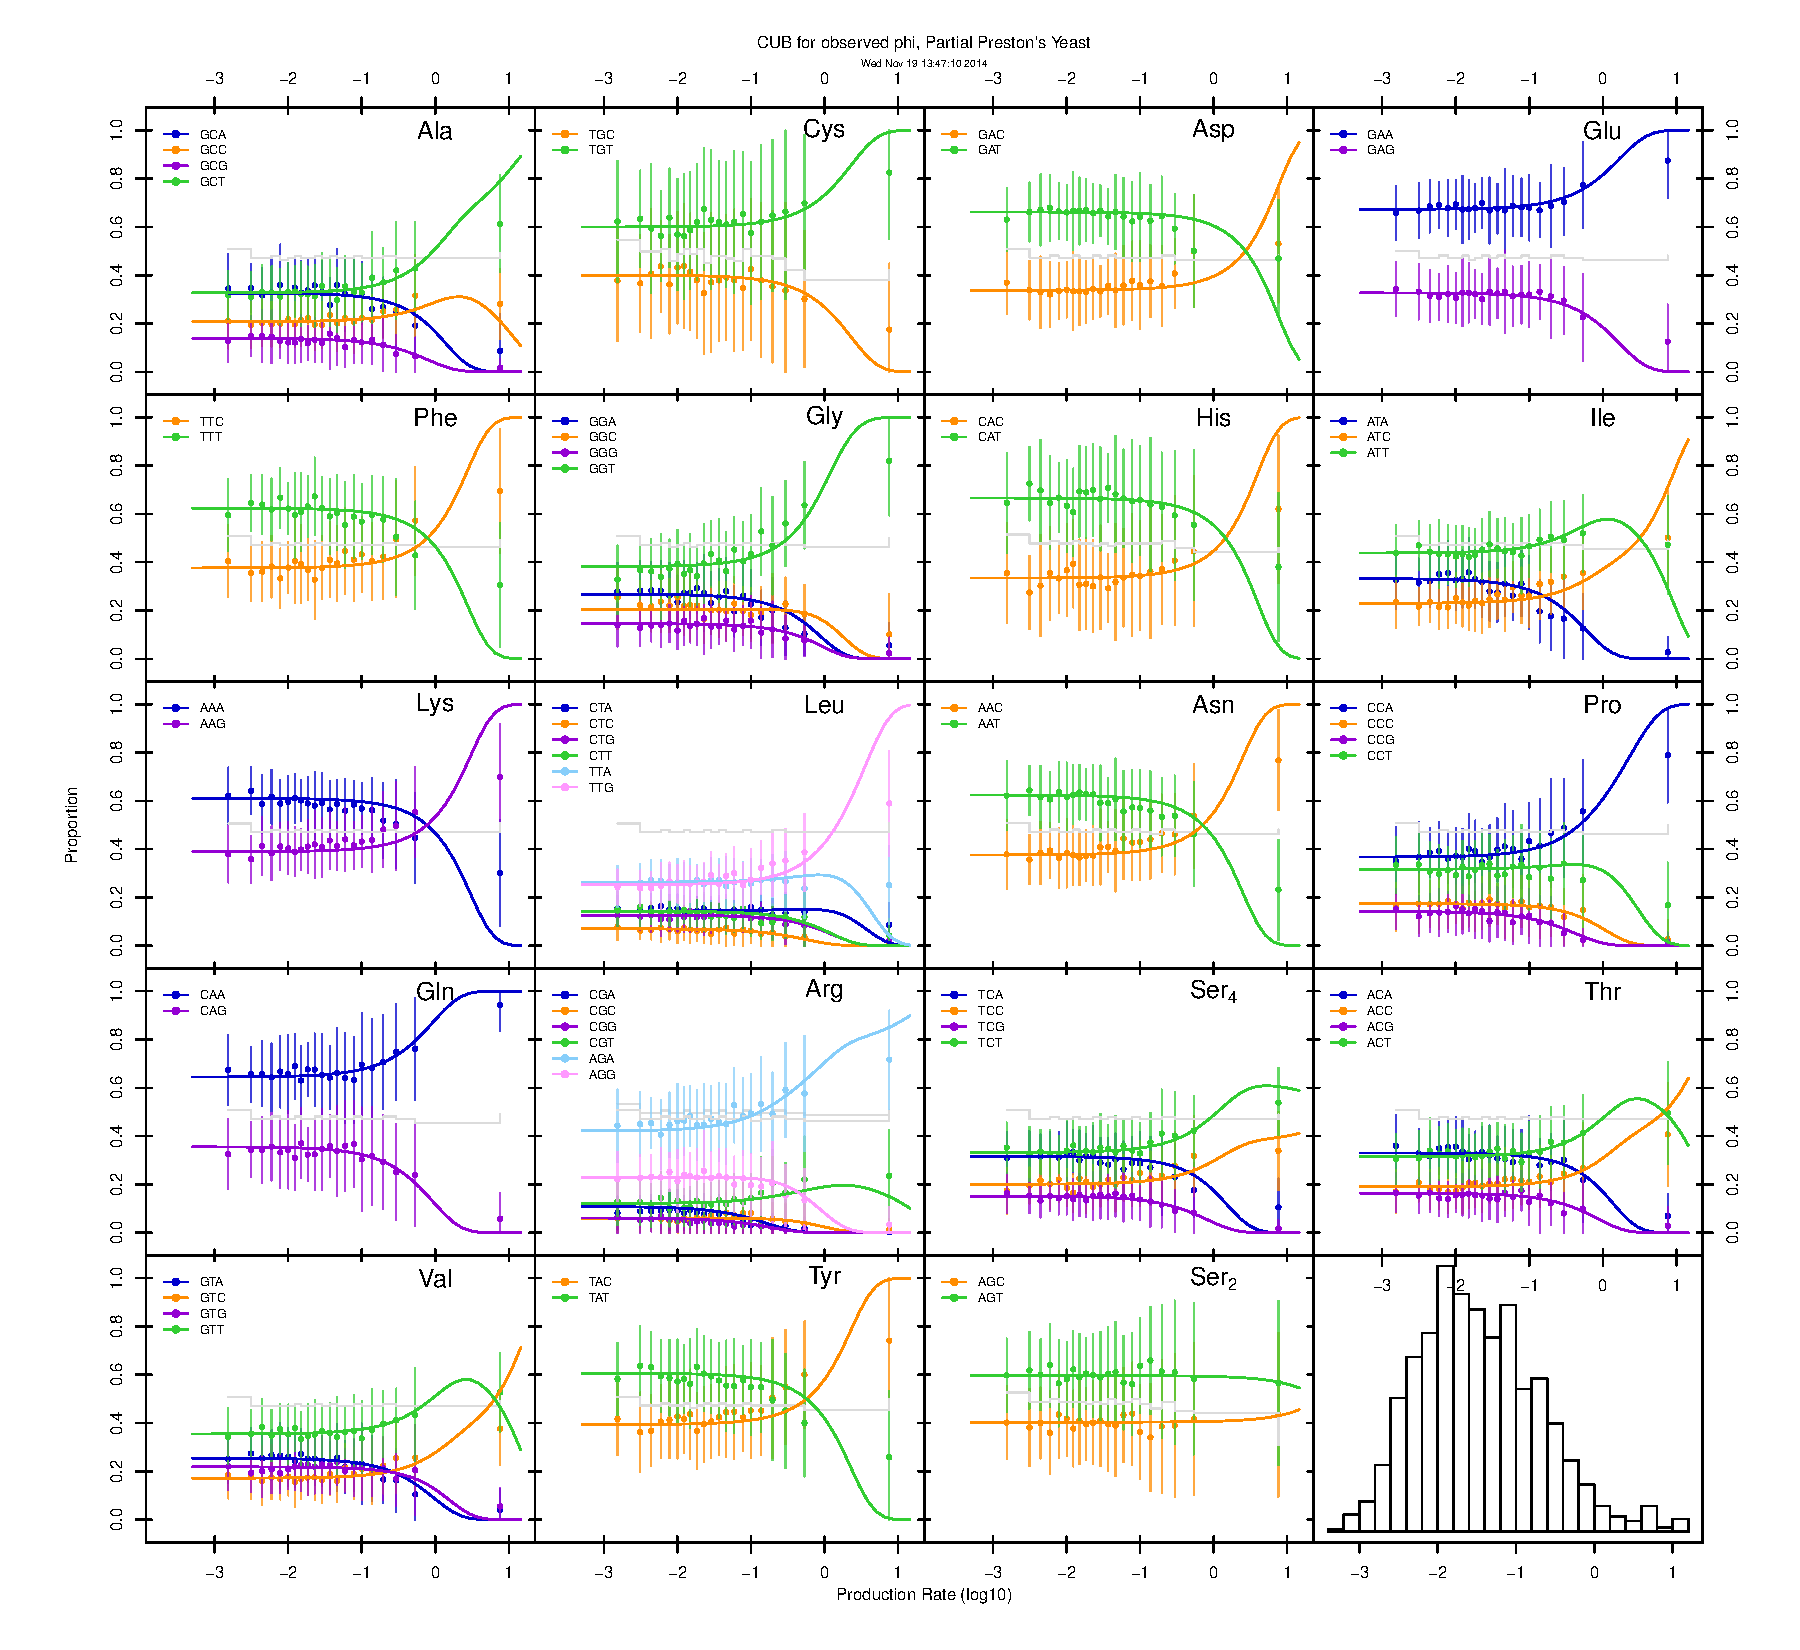
\includepdf[pages={1}]{data/partialPrestonYeast-CUBobsPhi.pdf}
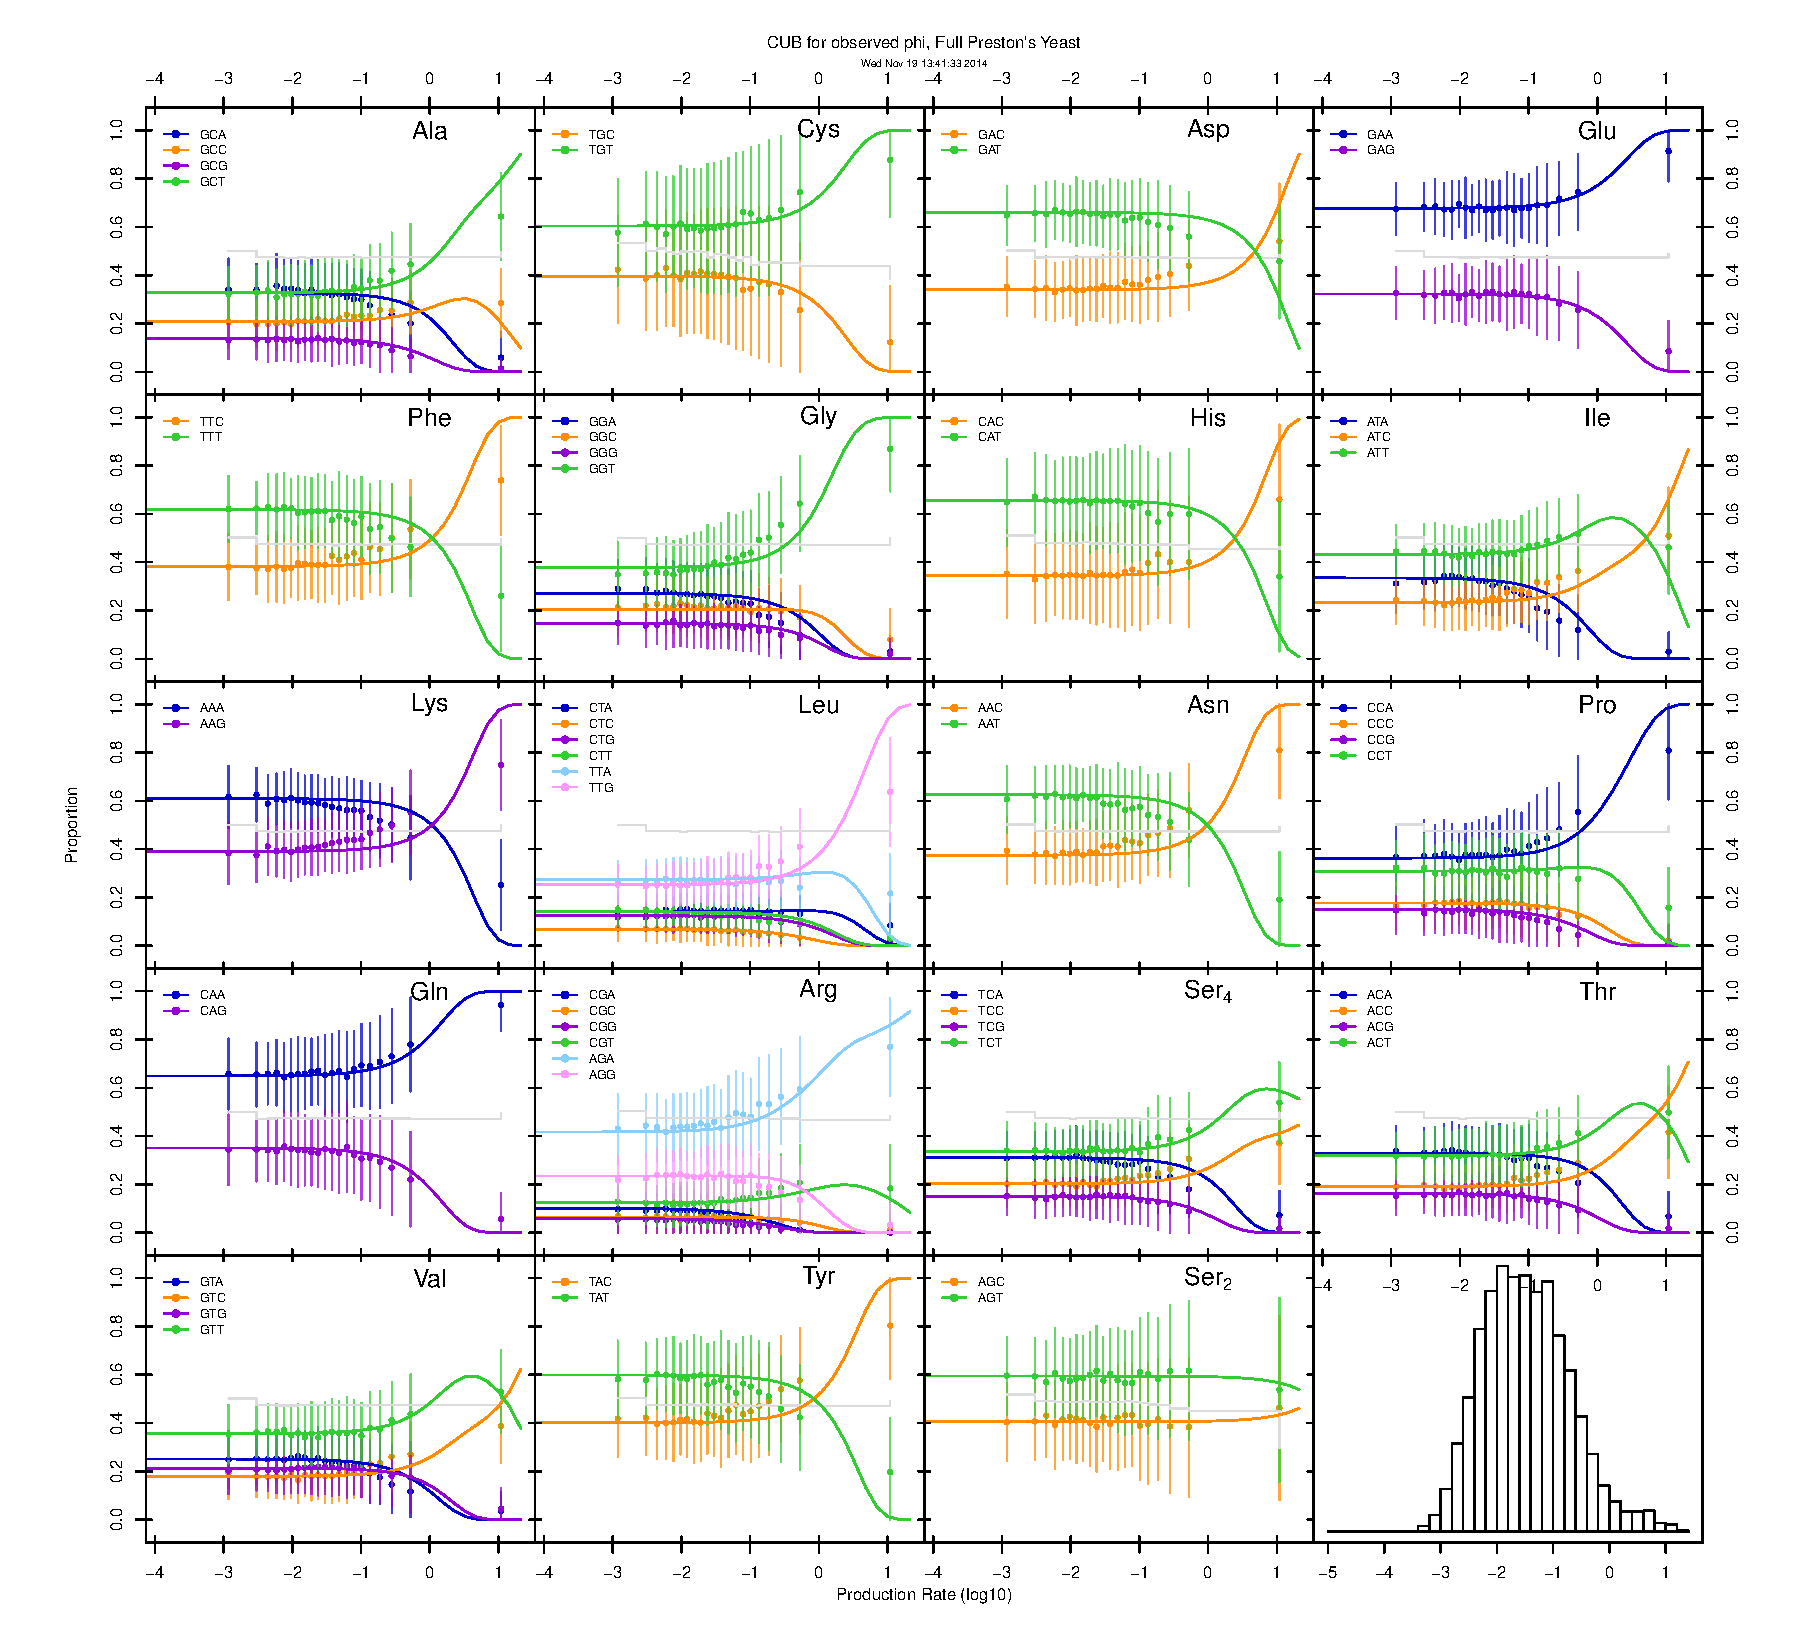
\includepdf[pages={1}]{data/fullPrestonYeast-CUBobsPhi.pdf}
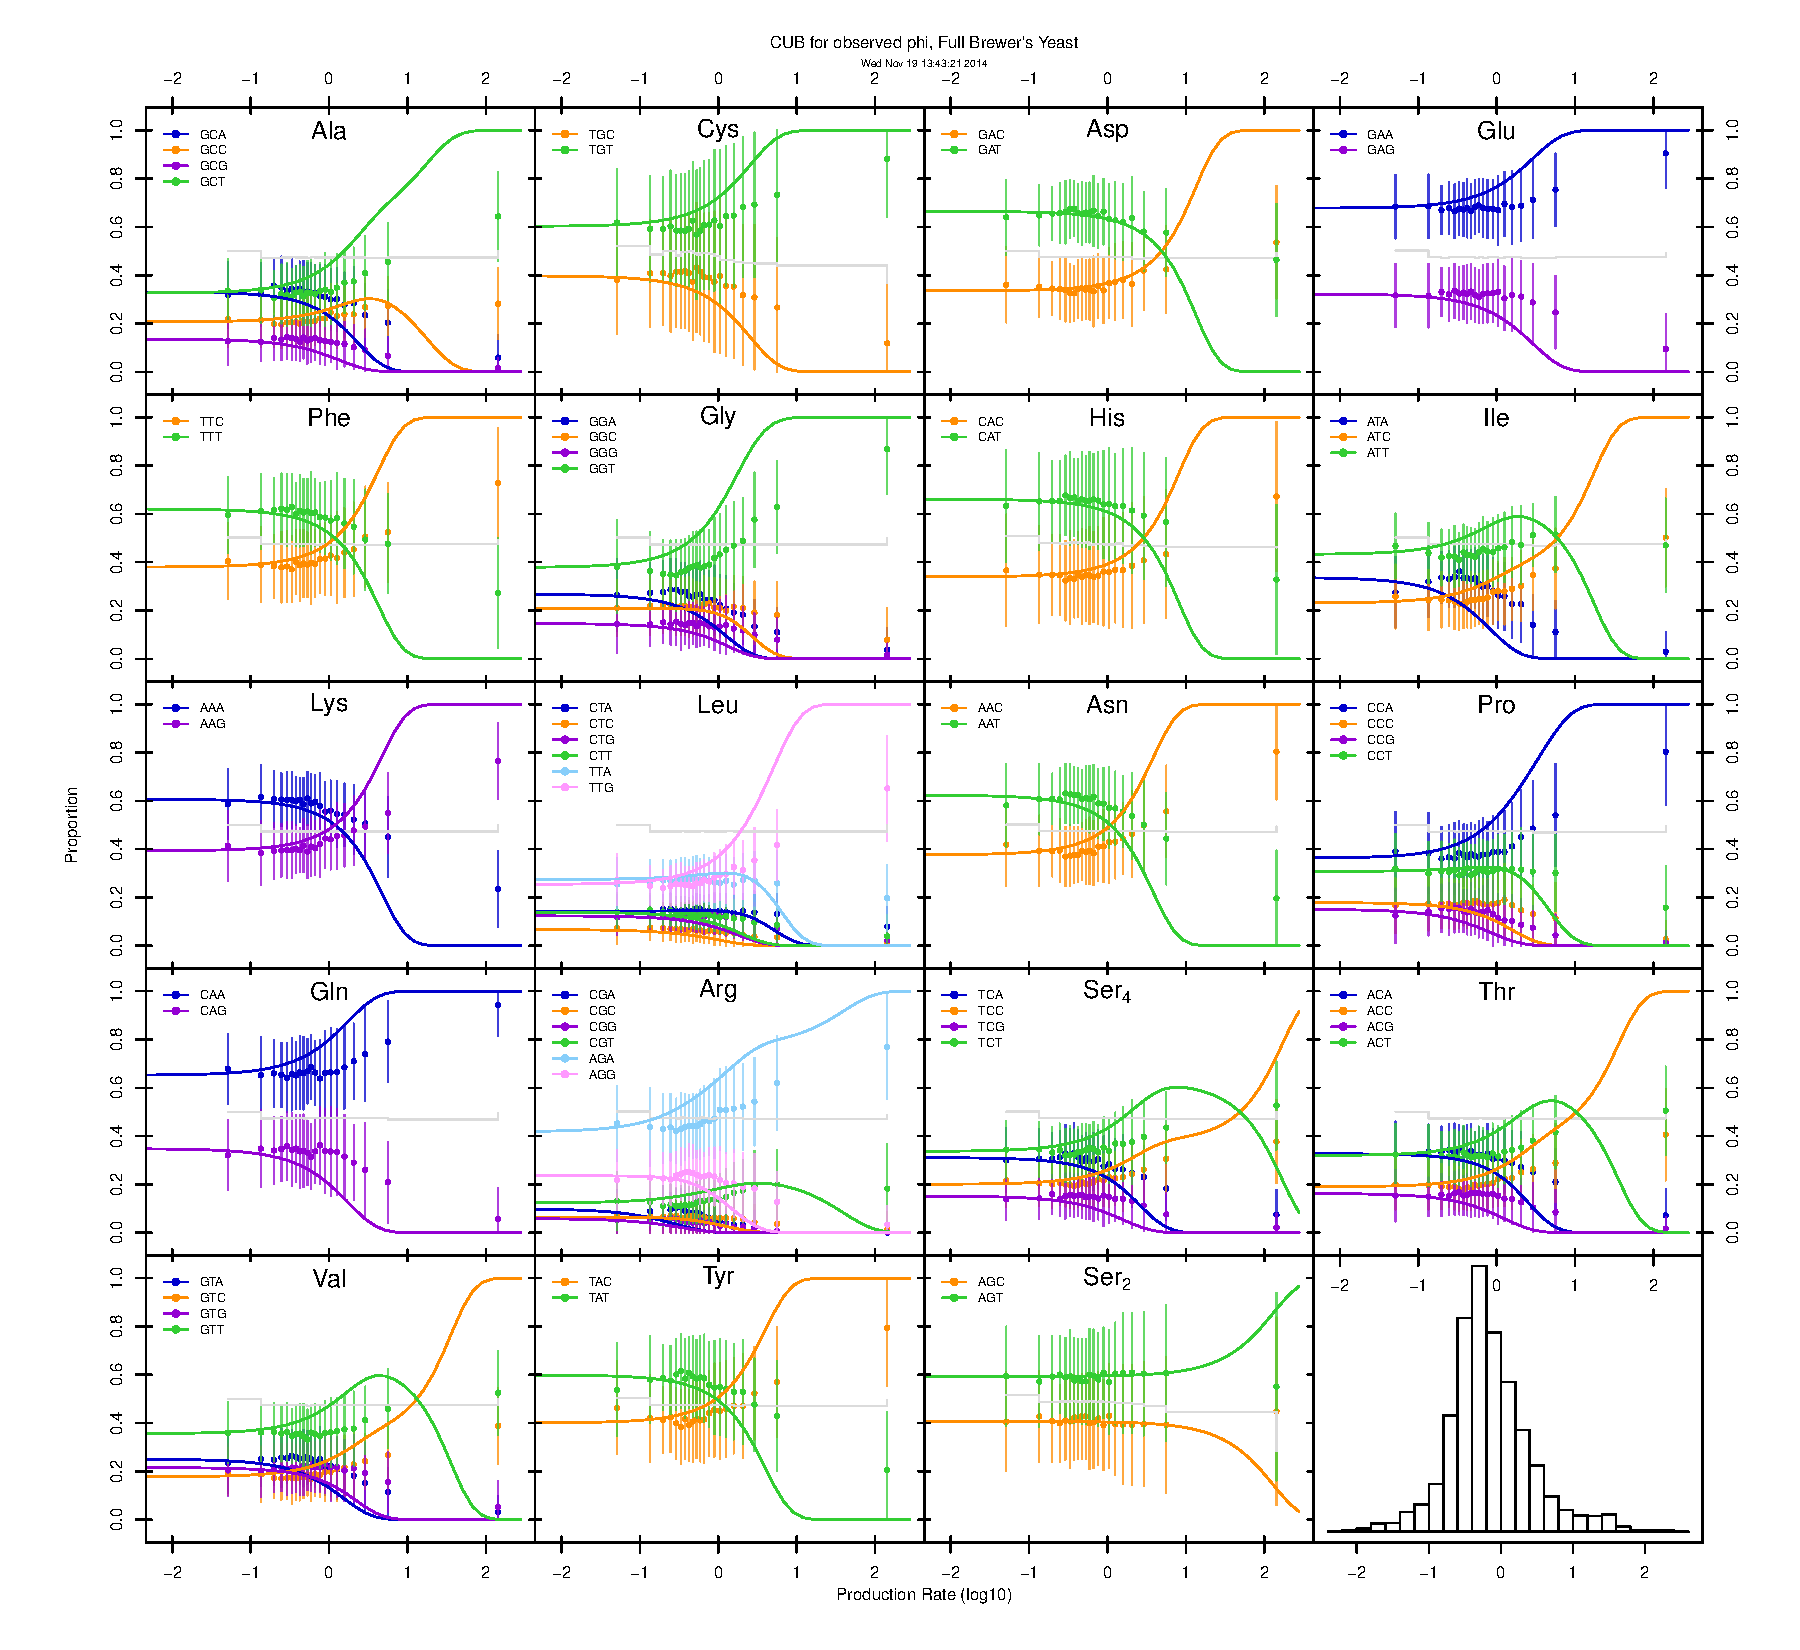
\includepdf[pages={1}]{data/fullBrewerYeast-CUBobsPhi.pdf}

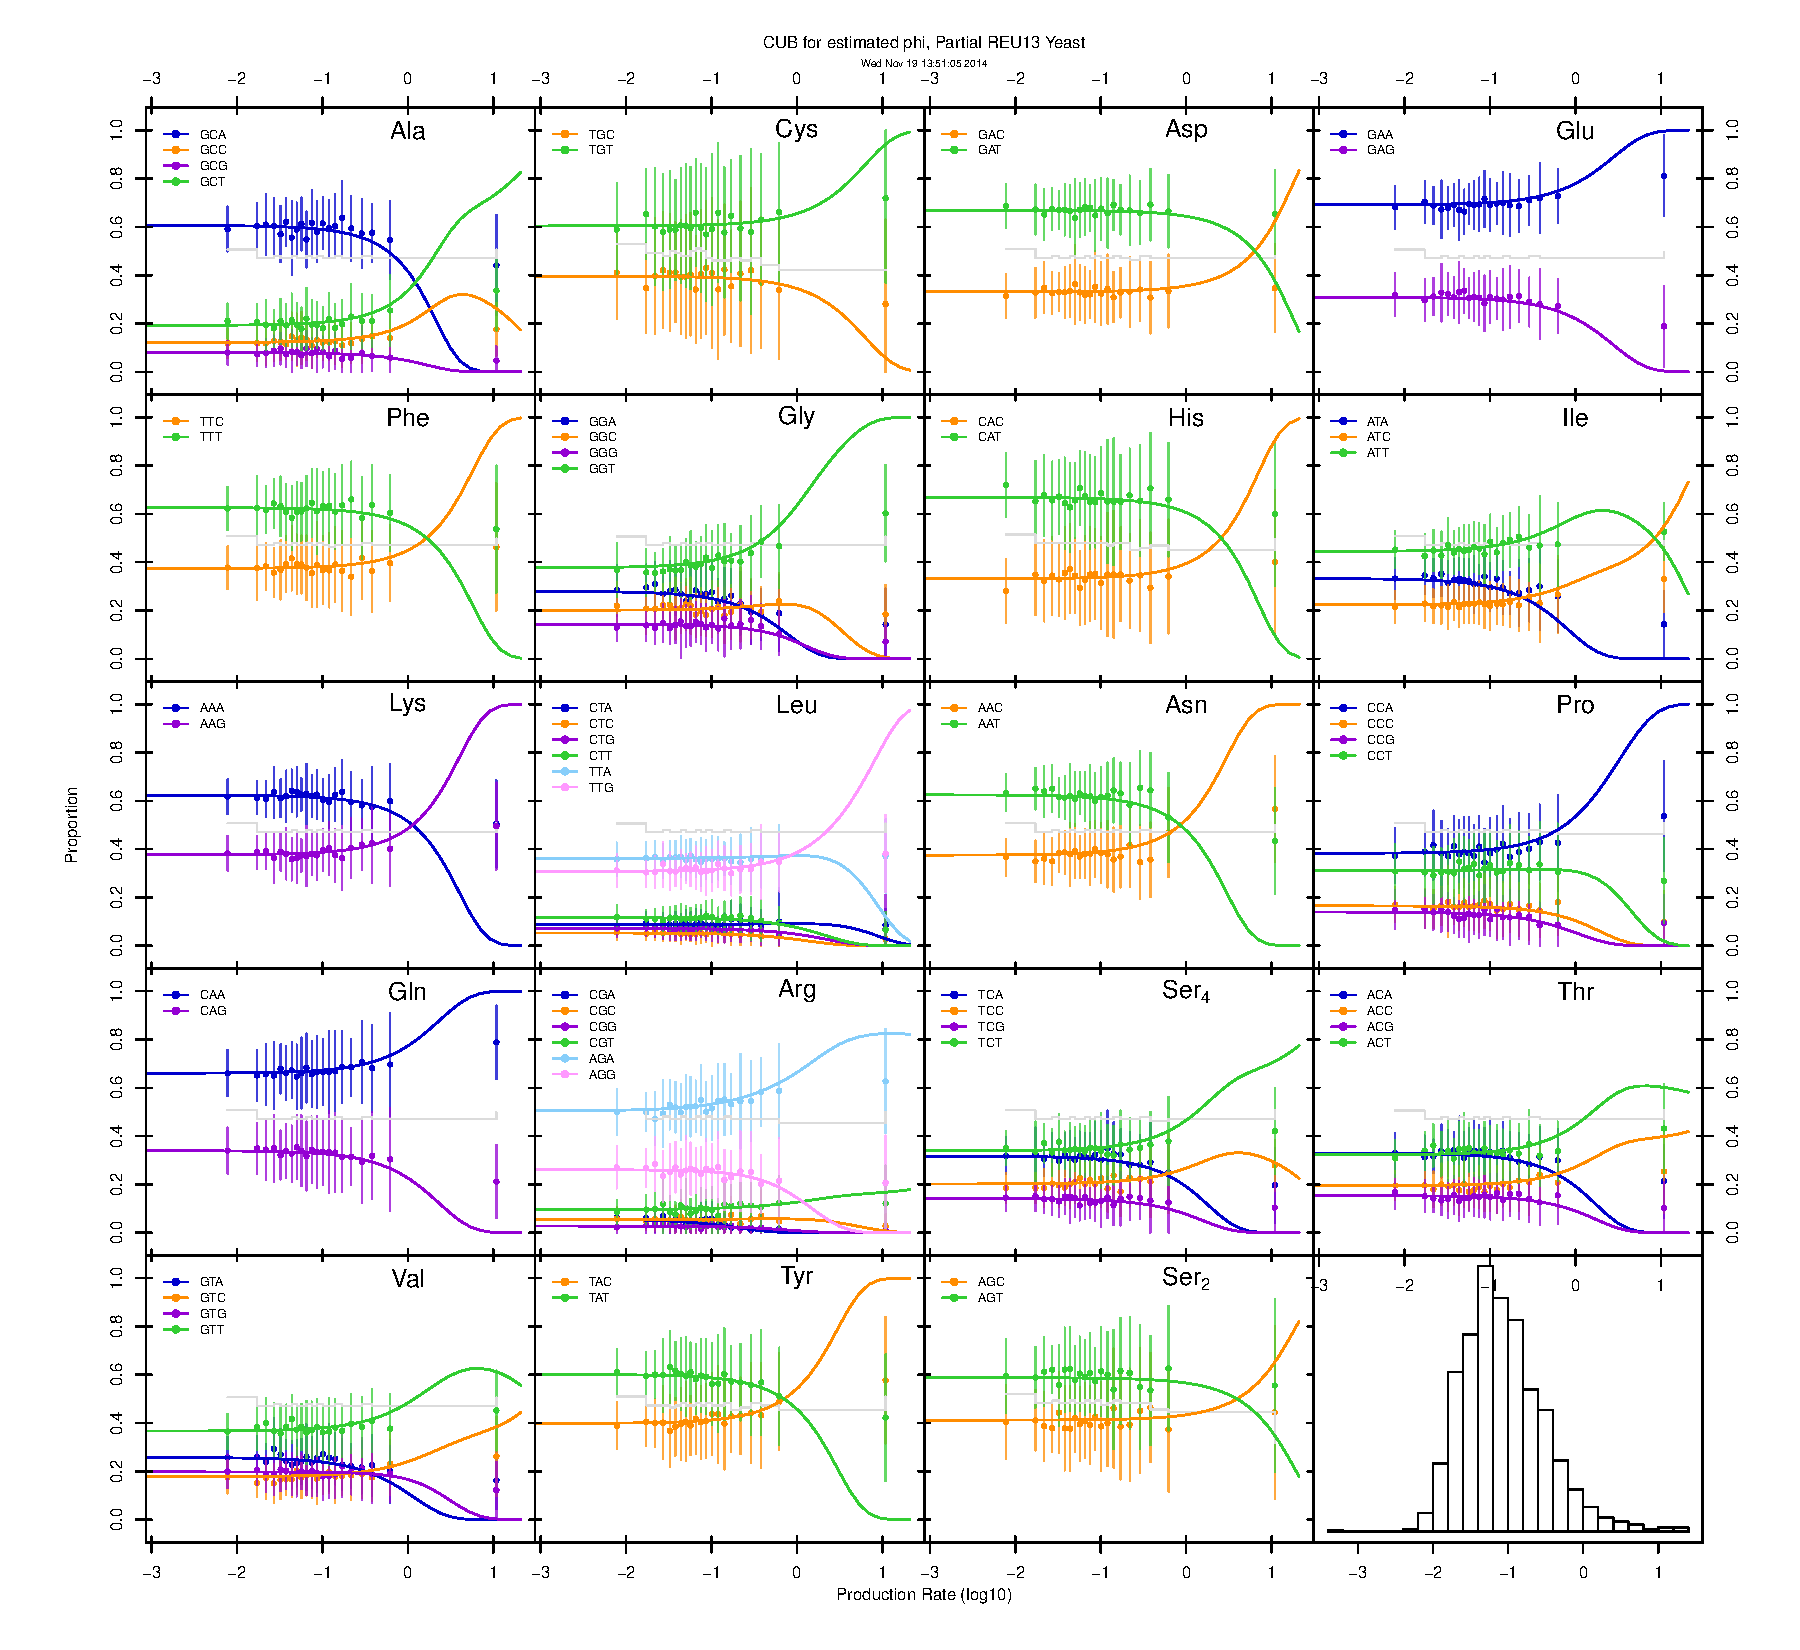
\includepdf[pages={1}]{data/partialREUYeast-CUBestPhi.pdf}
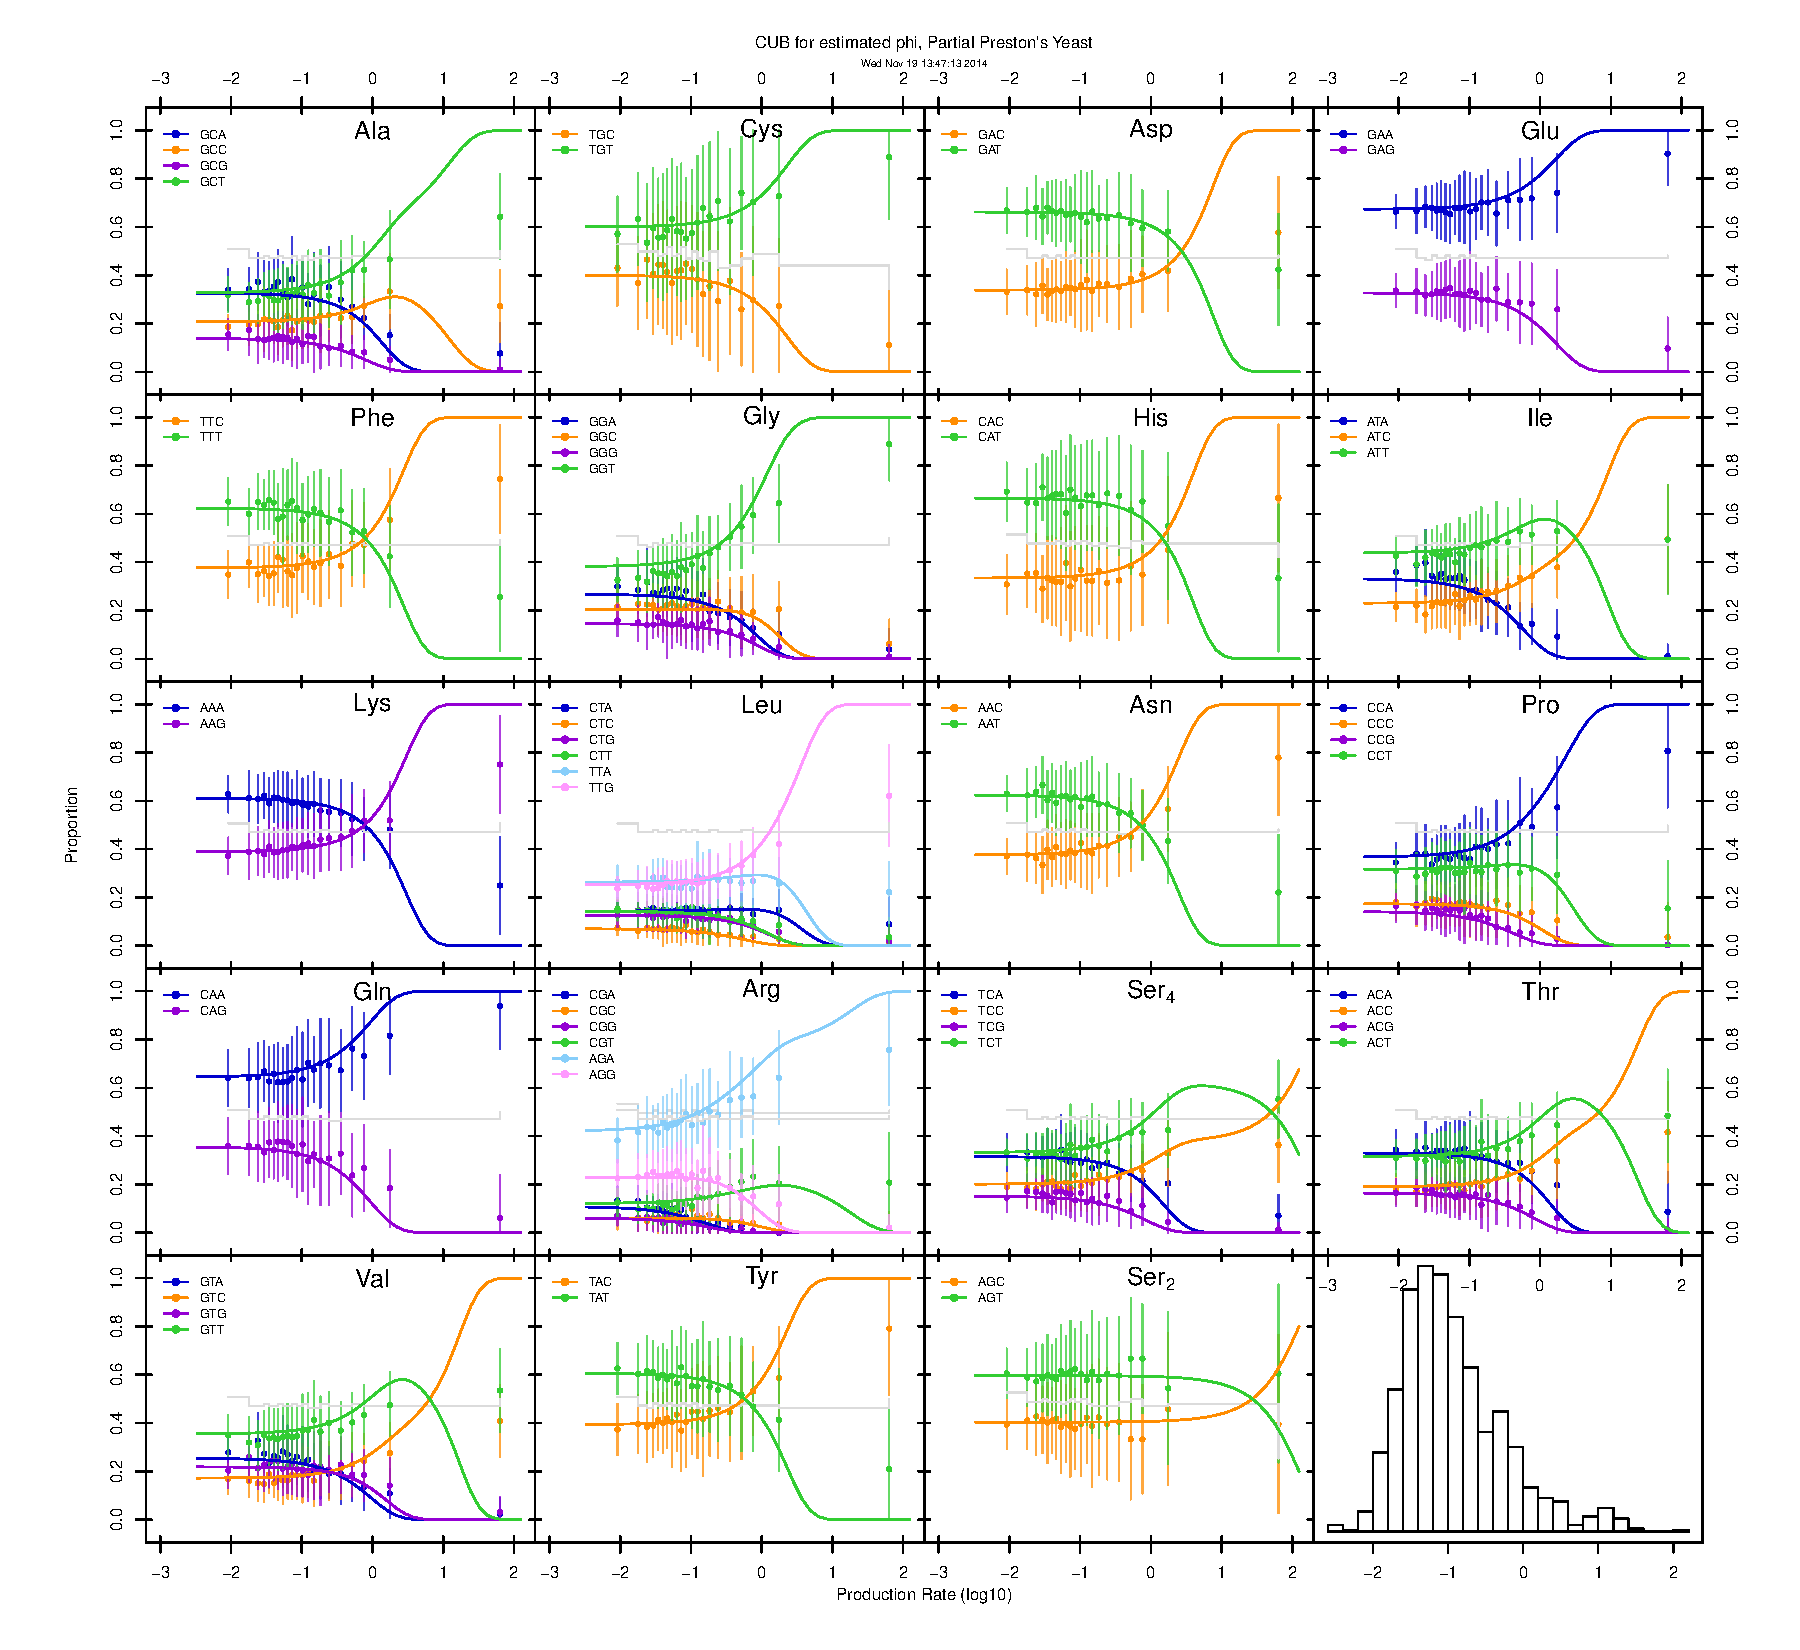
\includepdf[pages={1}]{data/partialPrestonYeast-CUBestPhi.pdf}
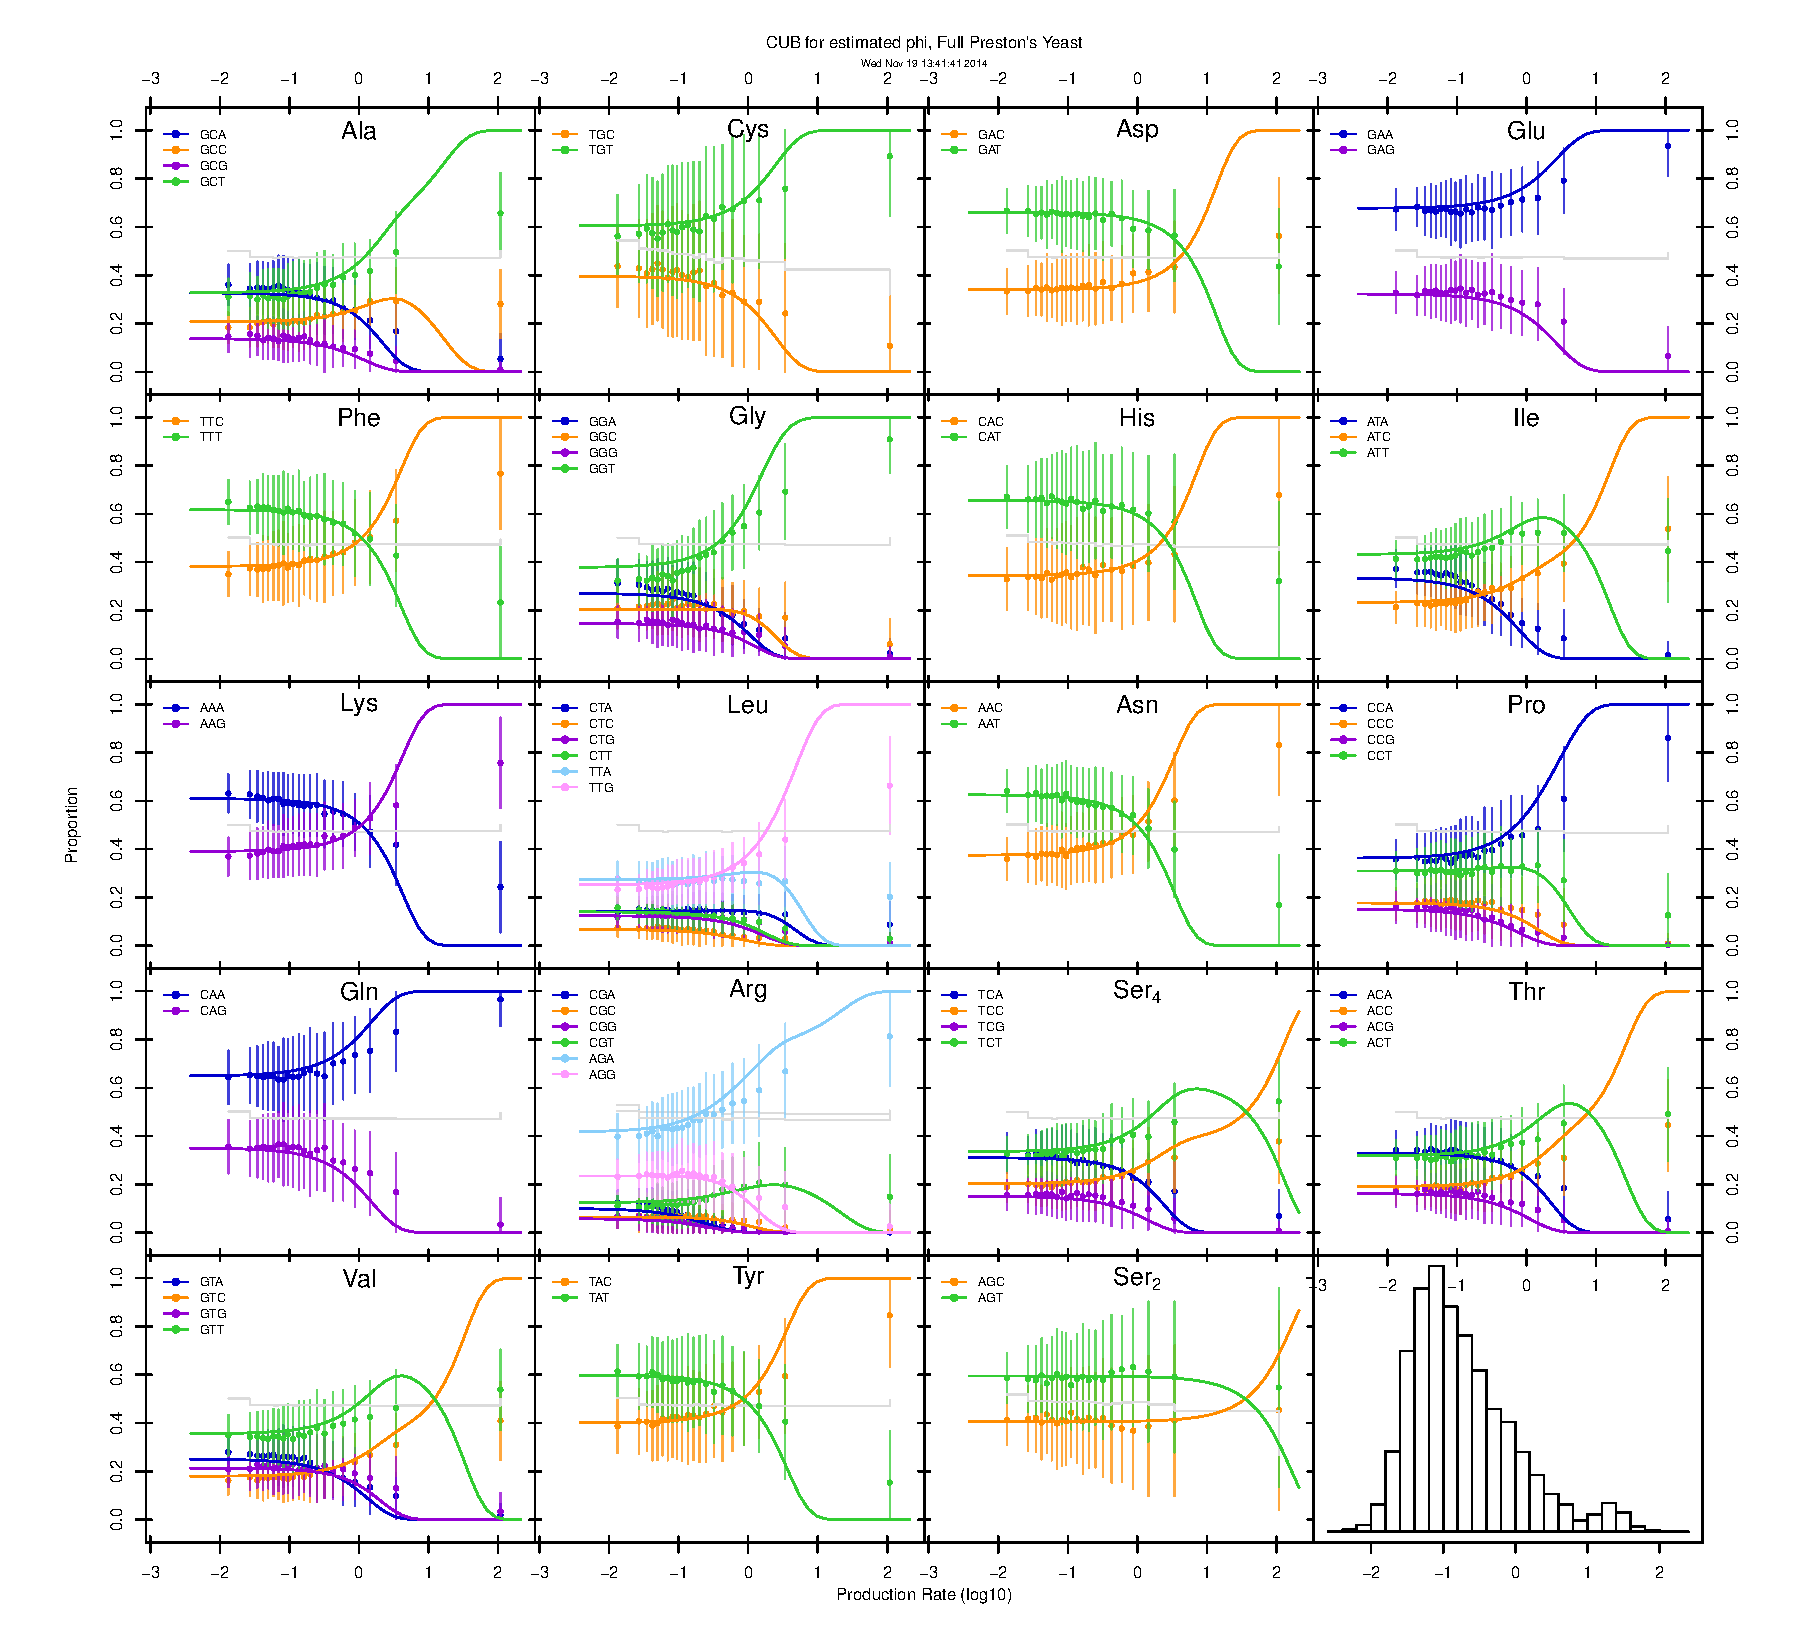
\includepdf[pages={1}]{data/fullPrestonYeast-CUBestPhi.pdf}
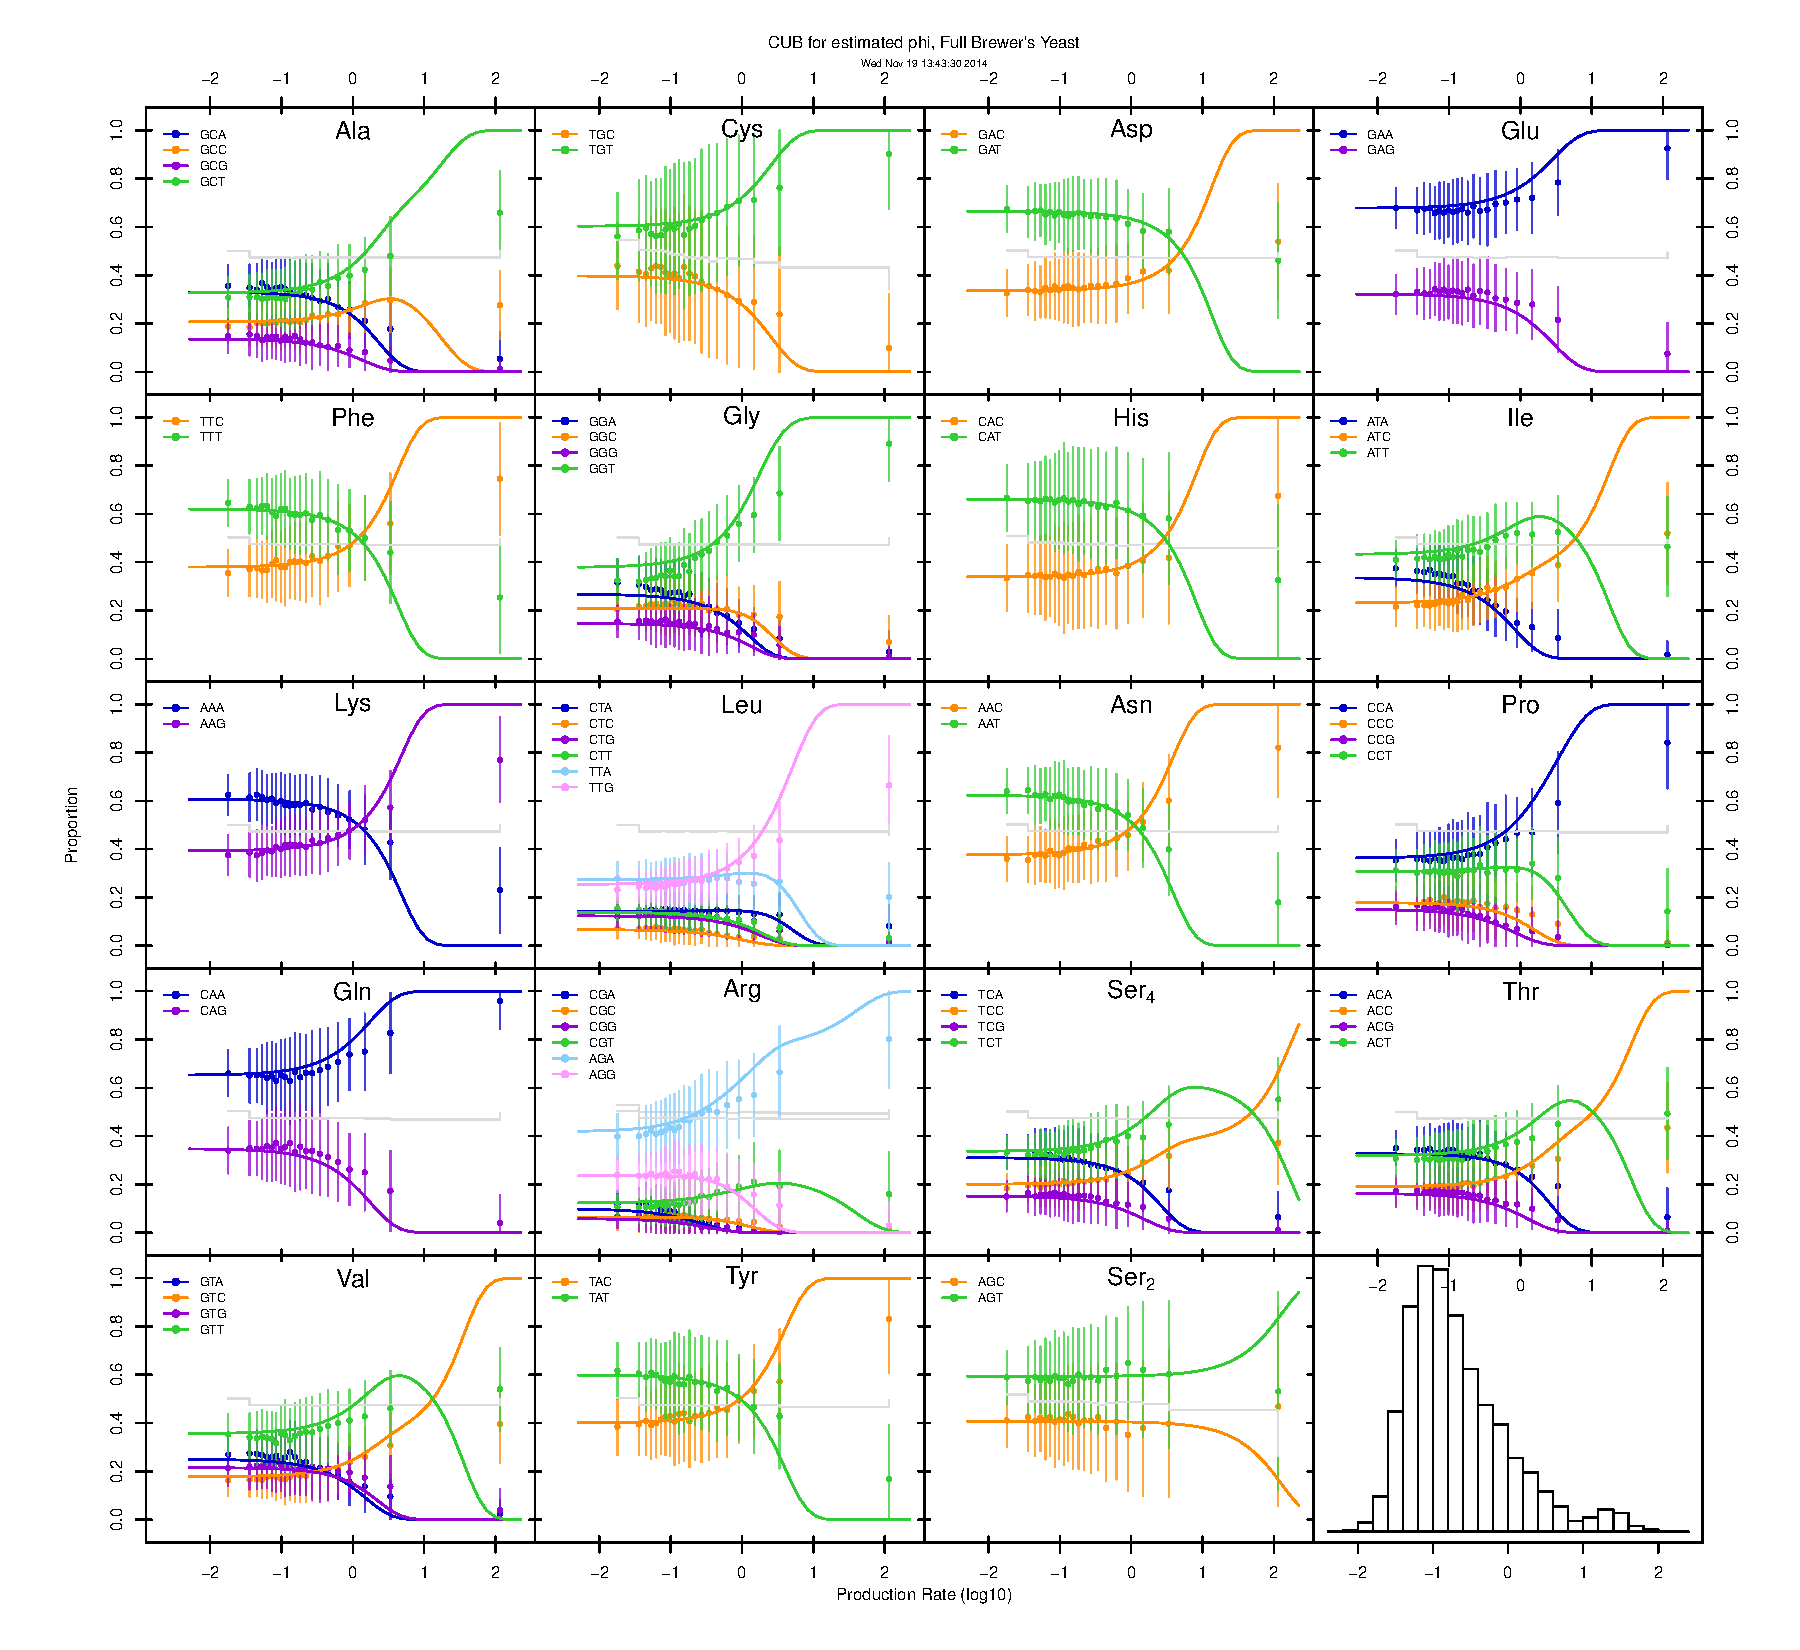
\includepdf[pages={1}]{data/fullBrewerYeast-CUBestPhi.pdf}


\subsection{Generate my own simulated yeast, using a reverse engineered cubfits}

Still an interest, but it's fallen down the priorities. The existing genomes seem to do fine.


\subsection{Parallelize the Code}

\subsubsection{getOption(``mc.cores")}
How to set the number of cores for an mclapply call? mclapply's default number of cores is getOption(``mc.cores",2L);

getOption(``(option)", (value)) returns the value previously set to that (option), or otherwise it returns (value). mc.cores is not set by default. So first, set option(``mc.cores"=Number\_of\_Cores). Then mclapply should correctly get the number of cores.

\subsubsection{Timing}

As expected, we get diminshing returns on adding additional processors

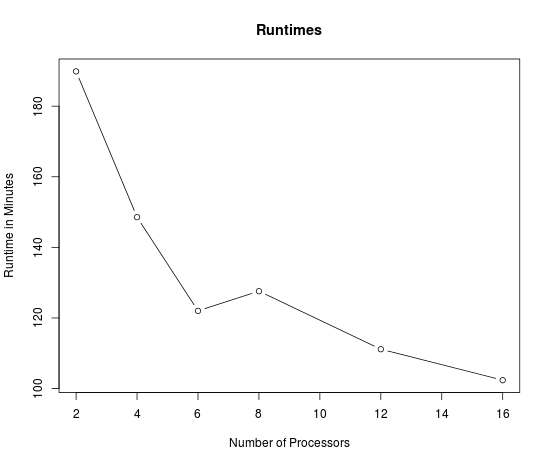
\includegraphics[width=0.5\textwidth]{data/1105runtimes.png}
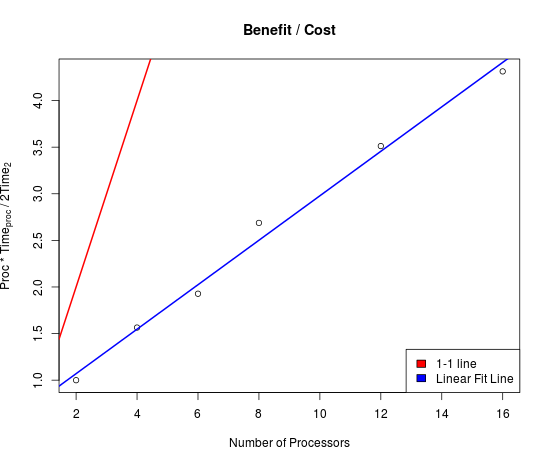
\includegraphics[width=0.5\textwidth]{data/1105timingCostBenefit.png}


\subsection{Change probability calculation}

Our results seem to indicate that the cost of a nonsense error is not high enough. The actual codon usage bias is not very high until you get to very high values of Phi. This doesn't match what we actually see.

In the code, when the posterior probability of a codon is calculated, instead of calculating

\[
\mbox{Pr}(c_i|\phi,i)
=
\frac{
\mbox{exp}[\mbox{M}_i
+ \omega_i(a_1-a_2)y_1
+ \omega_ia_2y_1 i
]
}{
\sum_{u=1}^m
\mbox{exp}[\mbox{M}_u
+ \omega_u(a_1-a_2)y_1
+ \omega_ua_2y_1 i
]
}
\]

Wei Chen calculates

\[
\mbox{Pr}(c_i|\phi,i)
=
\frac{
\mbox{exp}[\mbox{M}_i
%+ \omega_i(a_1-a_2)y_1
- \omega_i\phi i
]
}{
\sum_{u=1}^m
\mbox{exp}[\mbox{M}_u
%+ \omega_u(a_1-a_2)y_1
- \omega_u\phi i
]
}
\]

This was done for a number of reasons. The $y_1$ term is just the aggregate of the effective population, $\phi$, and a scaling term $-q$. Also, the assumption was that $a_1 \approx a_2 = 4$ATP.

\subsubsection{Adding $a_2$}

So it appears that Wei Chen never accounted for the direct cost of codon addition in the model. Maybe he was counting on it being cancelled by the scaling term $q$? In any case, I changed my.logdmultinomCodOne.r from
\begin{verbatim}
  xm <- matrix(cbind(1, tmp.phi * reu13.df.aa$Pos), ncol = 2)
\end{verbatim}

to

\begin{verbatim}
  xm <- matrix(cbind(1, 4 * tmp.phi * reu13.df.aa$Pos), ncol = 2)
\end{verbatim}

Since $a_2\approx4$.

Then xm\%*\% baamat should be
$
\mbox{M}_i- 4\omega_i\phi i
\approx
\mbox{M}_i- a_2\omega_i\phi i
$
As intended.


Implementing the change seemed to have no significant effect on the model, with Preston's Yeast or the REU Yeast. The results of the former are in cubfits/misc/results/np/11-10/*4ATP.pdf, and the latter are cubfits/misc/results/ny/11-10/*4ATP.pdf

This is troubling. I'm subtracting out an additional $3\omega\phi * position$ from each mutation bias, and I'm seeing very little results in actual codon usage bias. I checked the calculations in the browser, and it's accurate. 

\subsubsection{$\Delta a_{1,2}$}

To better account for the parameters of the model, we're going to add another parameter called $\Delta a_{1,2} = (a_1 - a_2)$, and use

\[
\mbox{Pr}(c_i|\phi,i)
=
\frac{
\mbox{exp}[\mbox{M}_i
- \omega_i(\Delta a_{1,2})\phi
- 4\omega_i\phi i
]
}{
\sum_{u=1}^m
\mbox{exp}[\mbox{M}_u
- \omega_u(\Delta a_{1,2})\phi
- 4\omega_u\phi i
]
}
\]

The math part of the change takes place in my.logdmultinomCodOne.r, adding an extra row to xm and multiplying $\omega\phi\Delta a_{1,2}$, which is baa[2]*tmp.phi*(new parameter)

\subsubsection{How to set $\Delta a_{1,2}$}

Mike suggests a small stepsize, but the big question is, when to we increase or decrease $\Delta a_{1,2}$?

I could add it to the baa matrix, and set it using the same vglm call in myfitMulitnomialOne.r that fits the M and $\omega$ values, but then it would be different for each amino acid. Of course, I could do that, and then set all of them equal to the (max/min/mean/median) value for $\Delta a_{1,2}$, but is that a bad idea? Also, this would make our VGLM call take longer, and it would disrupt our ability to fit the parameters we are already fitting. Those parameters would also be fit relative to an AA-specific $\Delta a_{1,2}$, even though $\Delta a_{1,2}$ would not be AA-specific.

\subsection{Move to Newton}

Newton uses R 3.0.1, all my dependencies were build under 3.1.1. Newton HAS R 3.1.0, but not 3.1.1.


\subsection{Wrong Names}

It's not just a problem in the chain\$b.Mat data. It's in the my.fitmultinomOne.r


\subsection{Visualization}

\subsubsection{'true' values vs simulated values}

Changes have been added to visualize.r, based on other plotting functions.

I've added confidence intervals (the scale of the interval can bet set in visualize.r). Cedric didn't have any functions to do so, but I was able to apply the "plotrix" package. I've also installed that package to "/home/lbrown/cubfits/Dependencies/plotrix". Everyone else should have permissions on that directory, in case someone wants to use my edited visualize.r function.


\subsubsection{Fix plotCUB}

The plotCUB function right now is calculated based on the ROC model. For the estimated and observed bias, the lines do not line up with the means and confidence intervals.

plotCUB generates the line (called predict.roc) using the prop.model.roc function. It seems to be based on my.logdmultinomCodOne.r. I've made the appropriate changes. By correctly using the $\Delta\omega$ values as $\Delta\omega$ (and not $\Delta\eta$), and also multiplying through by the mean position of the amino acid, we actually see a Codon Usage Bias!

I've made the appropriate changes in plotCUB so that it can take $a_2$ and $\Delta a_{1,2}$ as arguments, and actually use them in predicing the CUB for the NSE model. Right now, it takes the position as the mean position of that amino acid, which for S. Cerivisiae tends to be $\approx$350. 

The problem should be fixed, and also, shouldn't interfere with running the ROC model.


\subsection{logMu flip}

So as a result of the deltaEta switch, the code was multiplying the $\Delta log(\mu)$ values by -1. As I've described above in the $x \%*\% baamat$ calculation, it actually ended up doing negative mu, and fitting that. To the credit of the model, it was actually just fitting the opposite. Previously, I would just flip the result before plotting it.

I've gone into the my.logdmultinomCodOne.nse function and flipped the $\Delta log(\mu)$ back at the codon probability calculation. The result looks nice so far.

To illustrate, compare these two runs:

\begin{figure}[h!]
\caption{The first figure is a run before the logMu flip. The second is after. The second image has very small changes in $\Delta log(\mu)$, which looks like a more convincing result to me. Look especially at Glycine, at the purple line (codon GGG). Before the logMu flip, it started at about -1.2, went to 1.2, then converged around 1. After the flip, it started around -1.2, and converged around -1.}
\begin{tabular}{c|c}
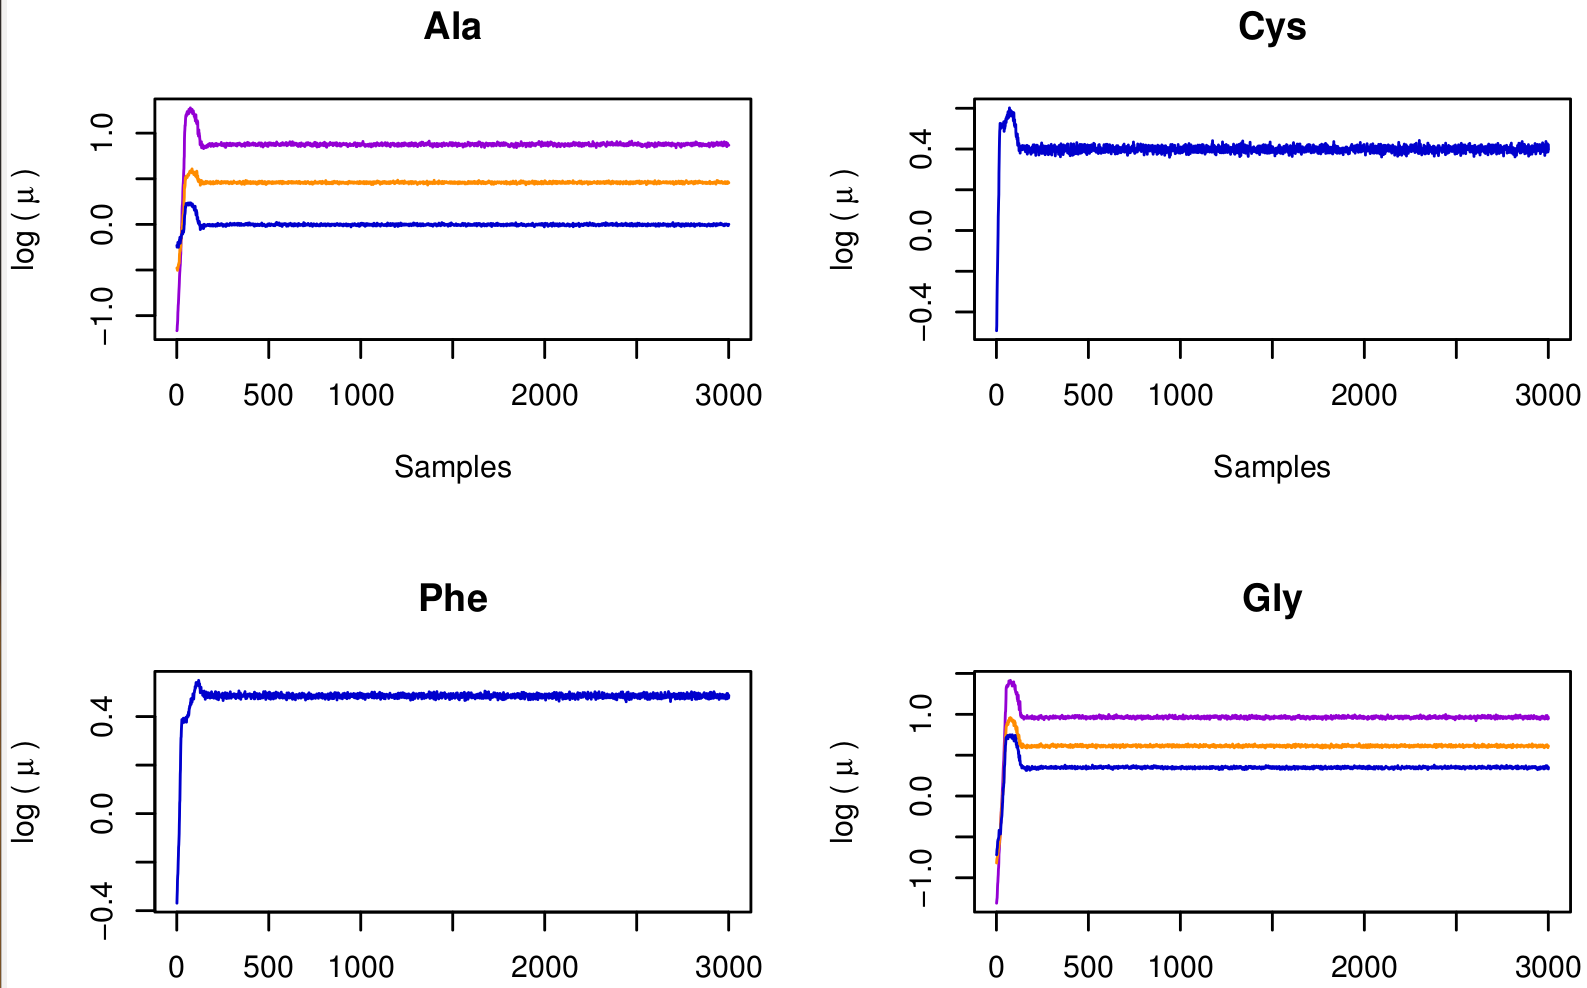
\includegraphics[width=0.48\textwidth]{data/logmu-nomflip.png}
&
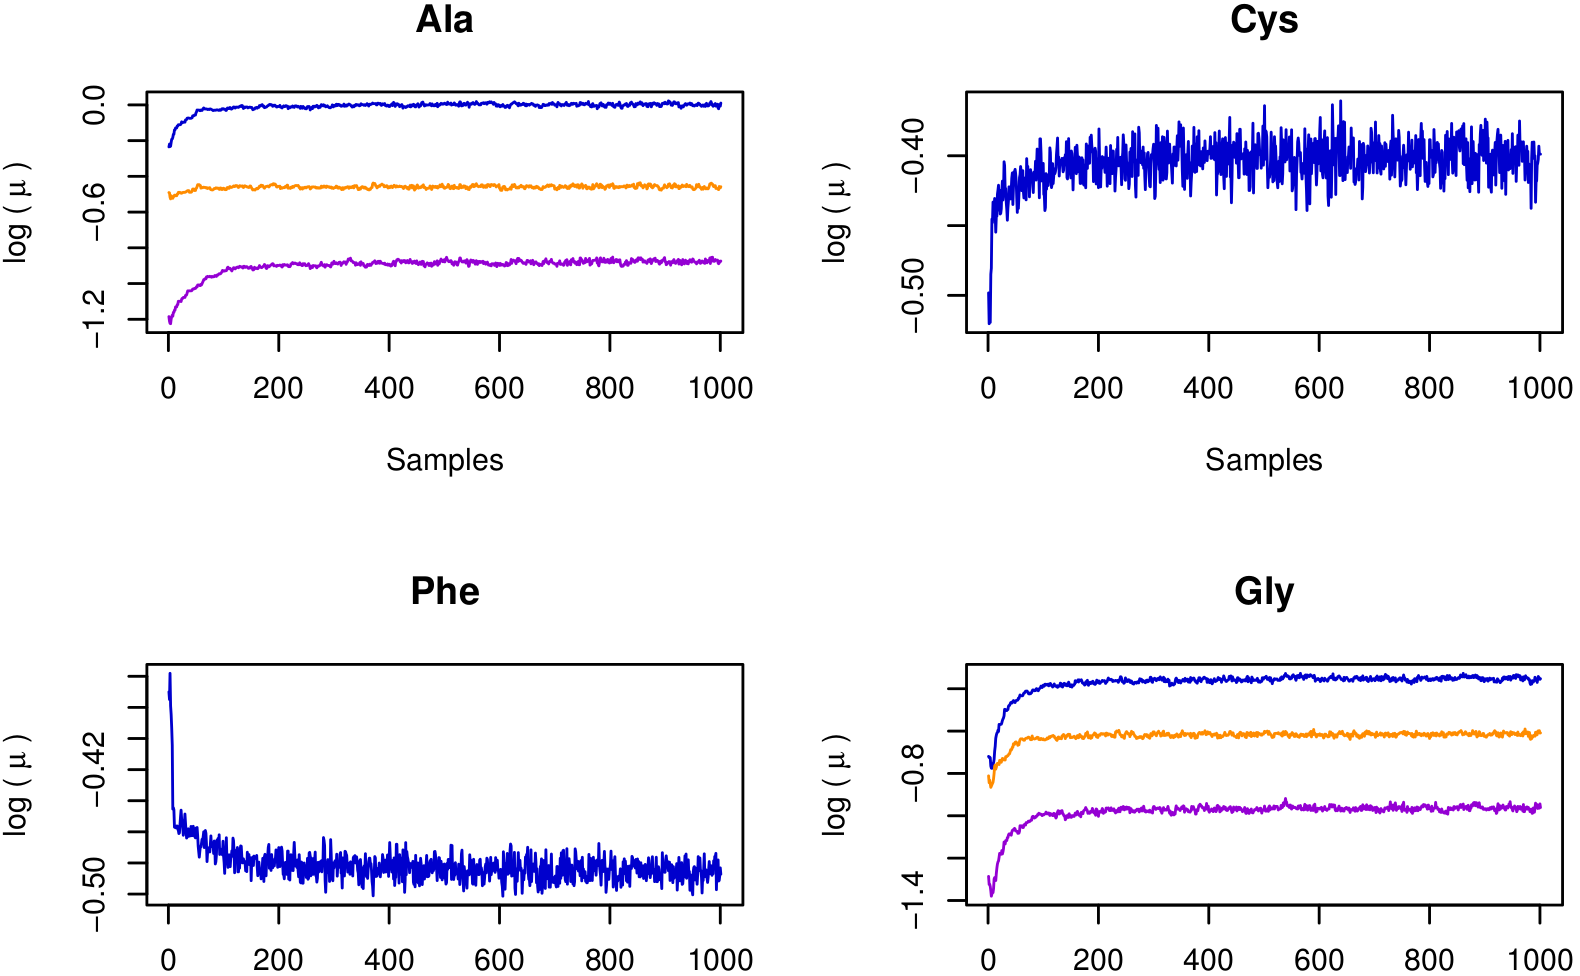
\includegraphics[width=0.48\textwidth]{data/logmu-mflip.png}
\end{tabular}
\end{figure}



\subsection{Problematic Codons}
There are a few codons that are consistently problematic between different runs.

These are the codons such that $|\mbox{estimated}\omega - \mbox{true}\omega| > 0.001$

\begin{verbatim}
   AA Codon  'true' omega  estm. Omega Occurances out of occurance rank   % Error
18  L   CTT  0.0024848544 0.0005788396      34288 268097          4 / 6 0.7670529
23  P   CCG -0.0006384656 0.0009225759      14920 121562          4 / 4 2.4449891
27  R   CGA  0.0003321017 0.0031227119       8543 124772          4 / 6 8.4028783
29  R   CGG  0.0010087399 0.0026759348       5067 124772          6 / 6 1.6527501
\end{verbatim}

These are the codons such that $$\frac{|\mbox{estimated}\omega - \mbox{true}\omega|}{|\mbox{true}\omega|} > 4$$

\begin{verbatim}
   AA Codon  'true' omega  estm. Omega Occurances out of occurance rank  % Error
9   G   GGC -5.892256e-05 0.0004492371      27742 140885          3 / 4 8.624195
27  R   CGA  3.321017e-04 0.0031227119       8543 124772          4 / 6 8.402878
\end{verbatim}


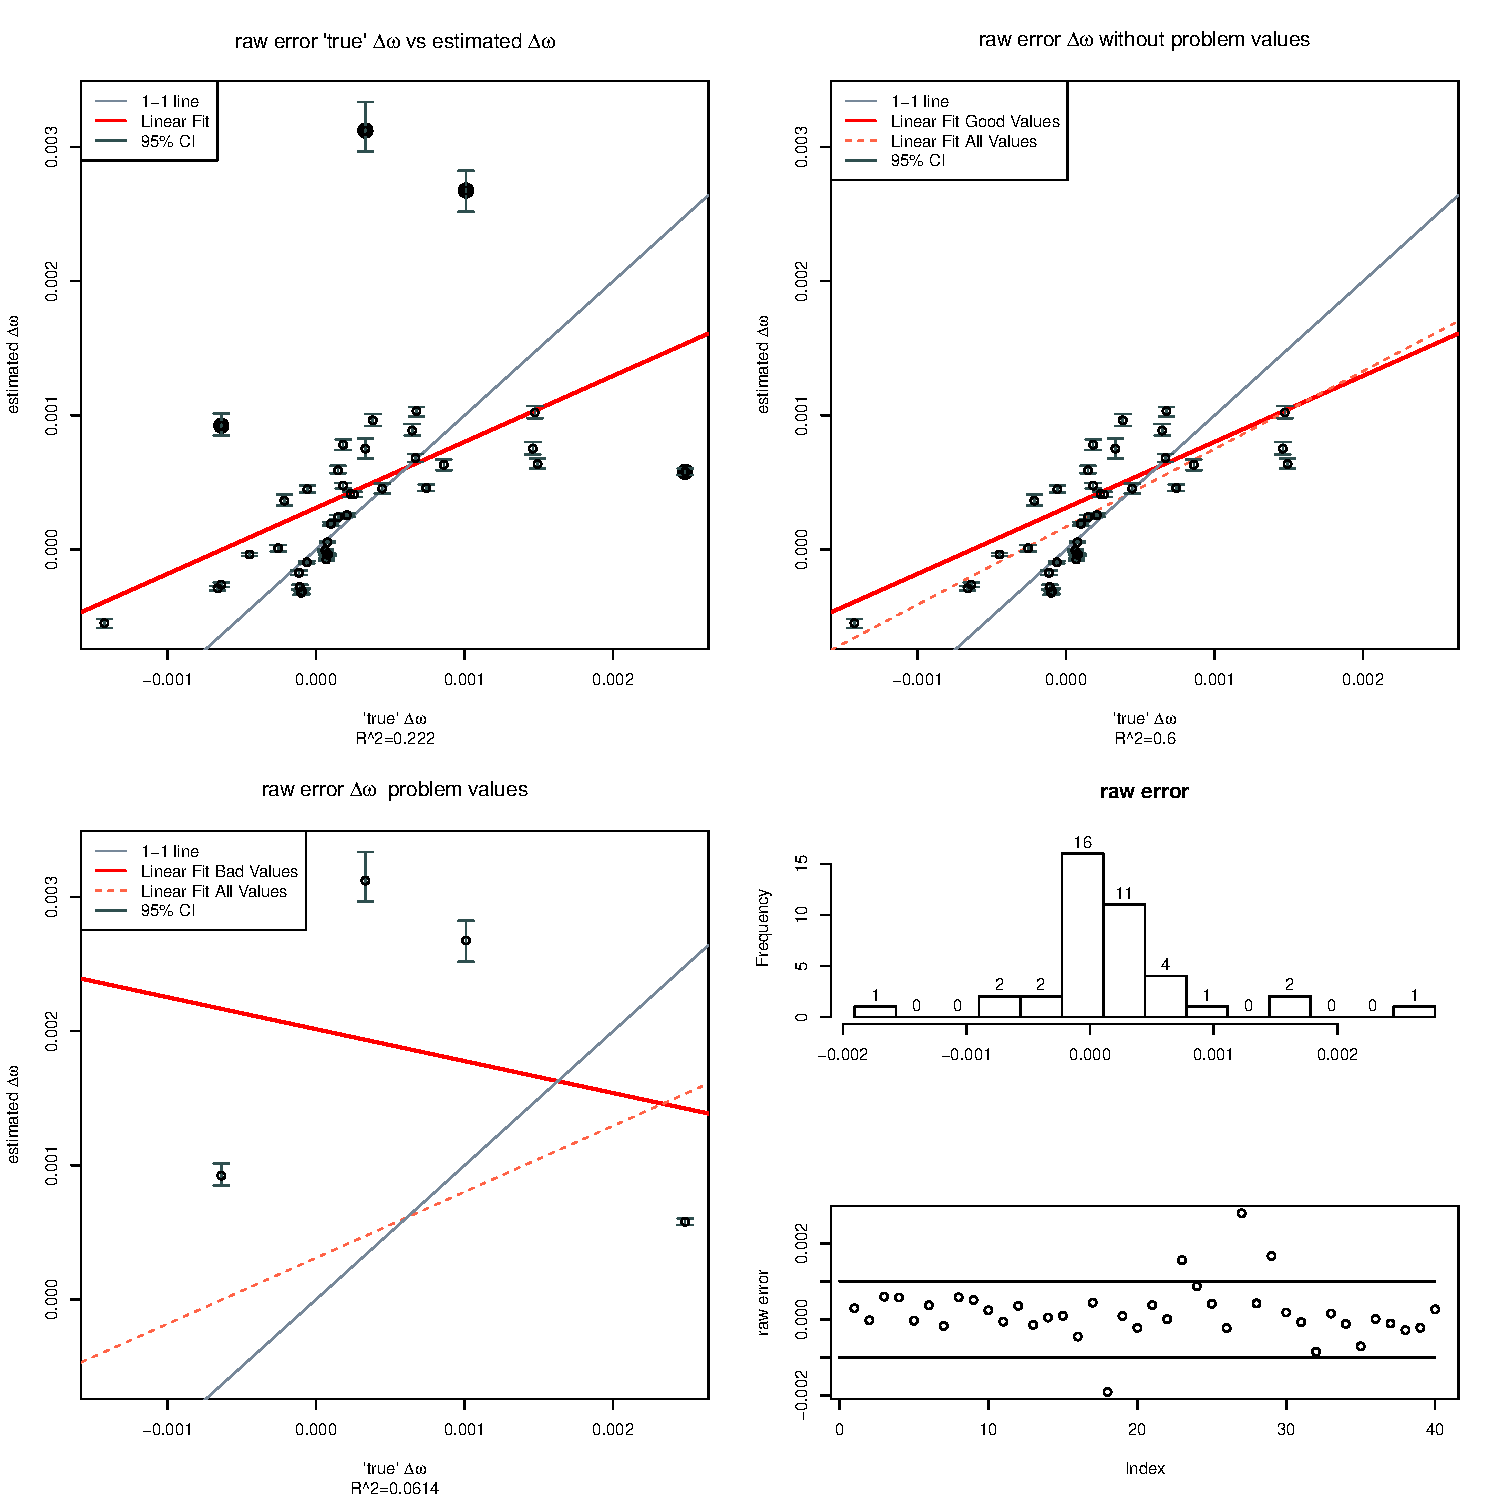
\includepdf[pages={1}]{data/omegastudy-RawError-1117.pdf}
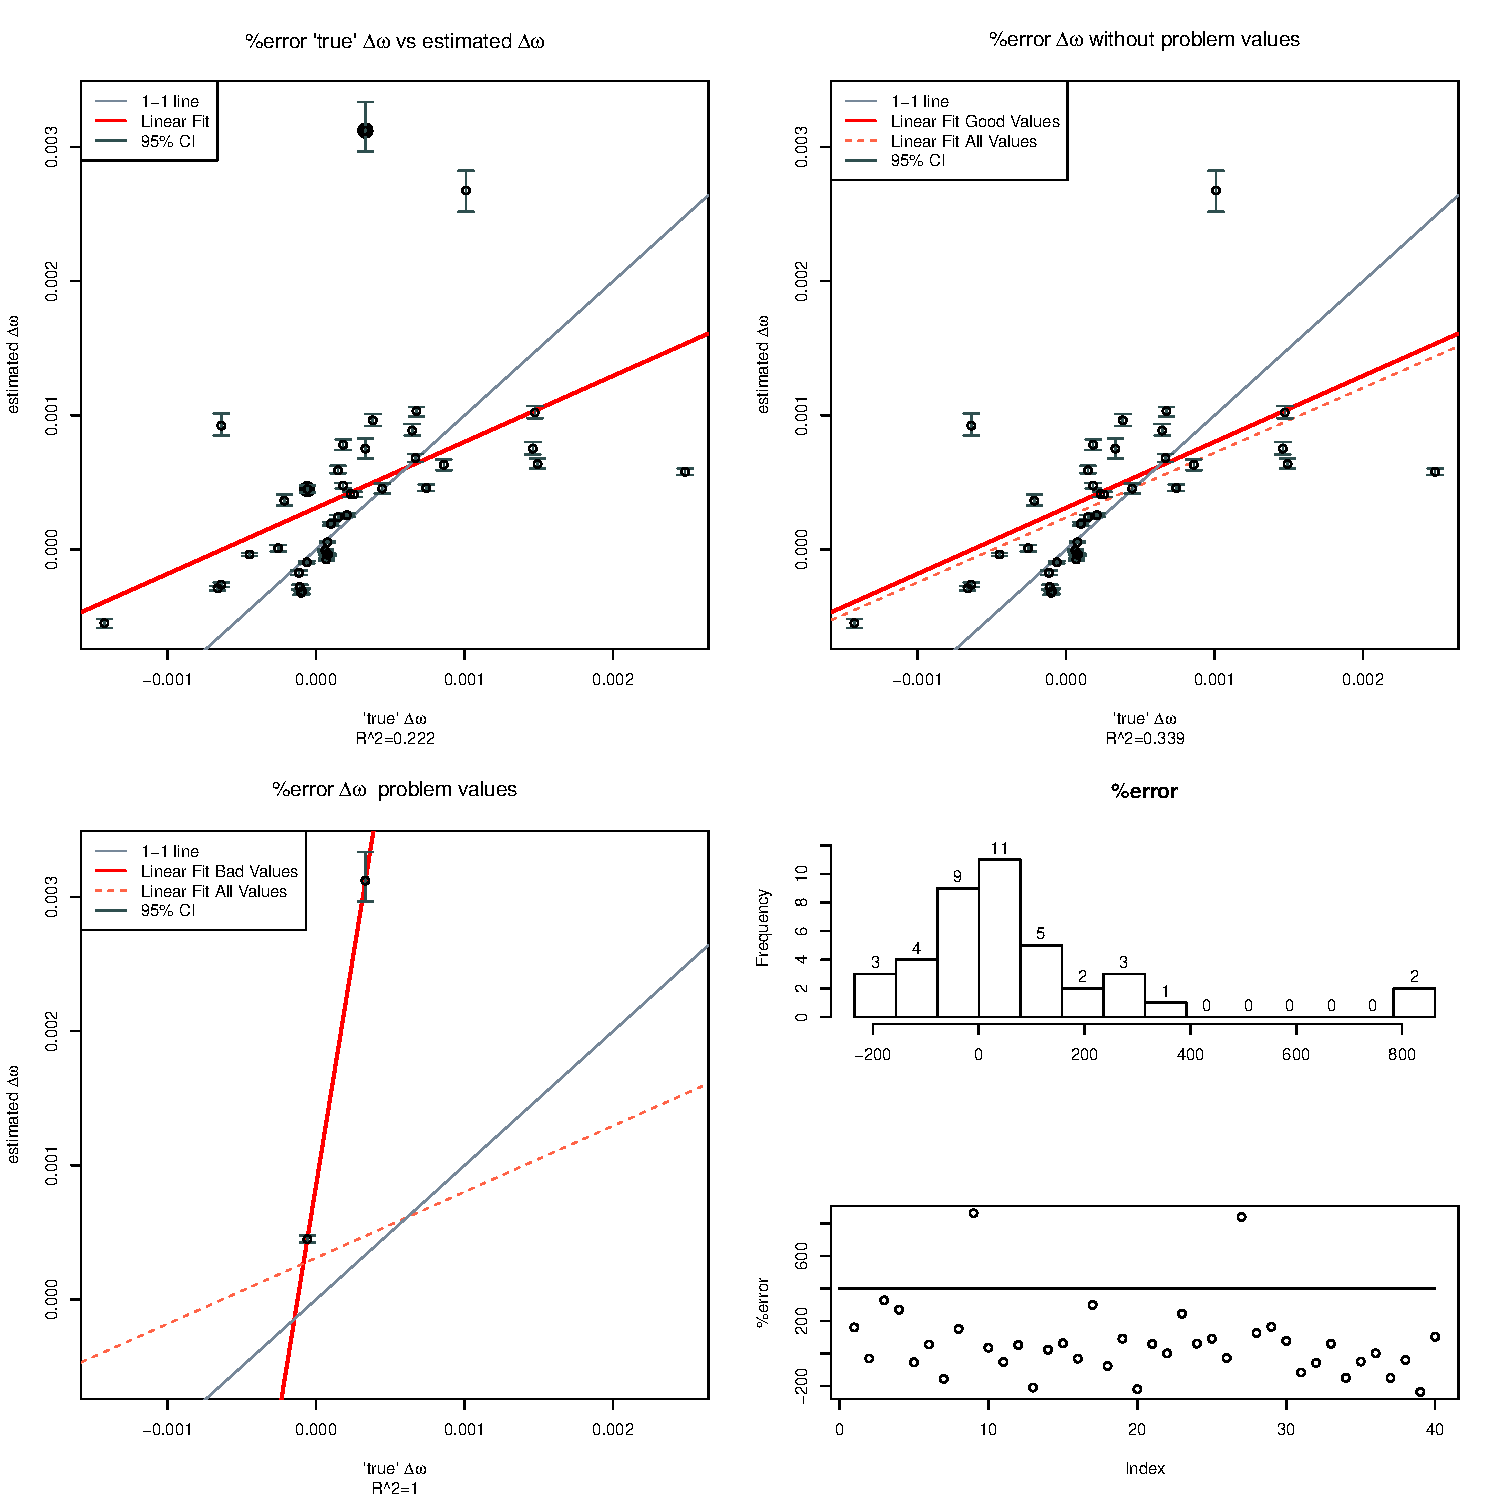
\includepdf[pages={1}]{data/omegastudy-PercentError-1117.pdf}

To me, it seems like the raw error is important. Percent error is a nice measure, but it unfairly picks out 'bad' values because they have small 'true' $\omega$ values.

\section{Goals for next Month}
\begin{enumerate}
\item Verify logMu Flip by larger runs
\item Problematic Codons
\item Is it worth it to adjust Delta a\_12?
\item Fix Names
\item Move to Newton?
\end{enumerate}


\end{document} %End of day document, REMOVE
